Esta seção apresenta as técnicas empregadas na construção dos métodos propostos de segmentação e classificação. Inicia-se definindo o conceito de imagem digital, em seguida são definidas as técnicas de Limiarização, Binarização, Limiarização Otsu e as técnicas de Limiarização Adaptativa como, por exemplo, o método de Niblack, o método de Sauvola e o método de Limiaraização Adaptativa Gaussiana. Em seguida, são apresentados os conceitos de Morfologia Matemática Binária e Morfologia Matemática Cinza e algumas técnicas para obter as propriedades geométricas de objetos como área, perímetro e circularidade. Por fim, é apresentado os algoritmos de aprendizagem de máquina e o descritor de textura \textit{Local Phase Quantization} (LPQ).

\section{IMAGENS}
%\label{sextion:imagens}

Uma imagem é representada matematicamente por uma função $f(x,y)$ da intensidade luminosa em qualquer ponto de coordenada espacial $(x,y)$. Está função é o produto da interação entre a iluminância $i(x,y)$, que é a quantidade de luz que incide sobre o objeto, e as propriedades de refletância do próprias do objeto, $r(x,y)$ cujo valor exprime a fração de luz incidente que o objeto vai transmitir ou refletir \cite{pddii}. Matematicamente,

\begin{equation}
	f(x,y) = i(x,y) \cdot r(x,y),
\end{equation}
em que $i(x,y) \in (0,\infty)$ e $r(x,y) \in (0,1)$.

Uma imagem é dita digital quando $(x,y)$ são números inteiros do $\mathbb{N} \times \mathbb{N}$ e $f$ uma função que atribui um valor inteiro de nível de cinza  para cada par distinto de coordenadas. Portanto, uma imagem digital é uma função bidimensional cujas coordenadas e valores de amplitude são números inteiros. Matematicamente, pode-se representar uma imagem digital como uma matriz, isto é, 

\begin{equation}
	f(x,y) = \begin{bmatrix}
		f(0,0) &   f(0,1) & \cdots & f(0,N-1) \\
		f(1,0) &   f(1,1) & \cdots & f(1,N-1) \\
		\vdots &   \vdots & \ddots & \vdots   \\
		f(M-1,0) & f(M-1,1) & \cdots & f(M-1,N-1)
	\end{bmatrix},
\end{equation}
em que $f(0,0)$, $f(0,1)$, $\dots$, $f(M-1,N-1)$ são os valores inteiros de nível de cinza. Os elementos  $f(0,0)$, $f(0,1)$, $\dots$, $f(M-1,N-1)$ são chamados de elementos pictóricos, elementos de imagem ou \textit{pixels}. Neste texto, será adotado o nome \textit{pixels}. Os valores $f(0,0)$, $f(0,1)$, $\dots$, $f(M-1,N-1)$ pertencer ao intervalo $[L_{min},L_{max}]$. Por convenção, é comum deslocar este intervalo para o intervalo dos inteiros $[0, \gamma)$, sendo que o valor $0$ representa a cor preta e o valor $\gamma$ representa a cor branca \cite{gonzalezprocessamento}, \cite{pddii}.

No caso de imagens que possuem informações em bandas distintas, é necessário uma função $f(x,y)$ para cada banda. Por exemplo, imagens coloridas, padrão \textcolor{red}{R}\textcolor{green}{G}\textcolor{blue}{B}, possuem uma função para a banda vermelha (\textcolor{red}{R}ed), uma função para o banda verde (\textcolor{green}{G}reen) e uma função para a banda azul (\textcolor{blue}{B}lue). \cite{gonzalezprocessamento}, \cite{pddii}.

\section{TÉCNICAS DE LIMIARIZAÇÃO}

A Limiarização é uma técnica aplicada nas imagens em tons de cinza e consiste em separar a imagem em duas ou mais regiões de interesse. Este processo de separação é realizado comparando os valores dos \textit{pixels} com valores estabelecidos pelo usuário, esses valores são chamados de \textbf{limiar} \cite{gonzalezprocessamento, pedrinischwartz}. Pode-se definir o processo de Limiarização para uma imagem em tons de cinza como:

\begin{define}[\textit{Limiarização}]
	Dada uma imagem $f(x,y)$ e $T_1$, $T_2$, $T_3$, $\dots$, $T_n$ $\in [0,255]$, números naturais\footnote{$\mathbb{N} = \{0,1,2,3,...\}$}, valores de limiares. A imagem $g(x,y)$ limiarizada é dada como:
	\begin{equation}
		g(x,y) =
		\begin{cases}
			l_1, & se \; f(x,y) < T_1 \\
			l_2, & se \; T_1 \leq f(x,y) < T_2 \\
			l_3, & se \; T_2 \leq f(x,y) < T_3 \\
			\vdots \\
			l_n, & se \; f(x,y) \geq T_n,
		\end{cases}
		\label{eq:limiarizacao}
	\end{equation}
	\label{def:limiarizacao}
\end{define}

\noindent em que $l_1$, $l_2$, $l_3$, $\dots$, $l_n$ são valores de tons de cinza que a imagem assumirá. Vale ressaltar que esses valores são escolhidos pelo usuário. A seguir é apresentado um exemplo aplicando a definição \ref{def:limiarizacao}.

\begin{exemplo}
	Seja dois limiares $T_1 = 100$ e $T_2 = 200$ e os valores de cinza $l_1 = 50$, $l_2 = 200$ e $l_3 = 230$ que a imagem pode assumir. A equação \ref{eq:limiarizacao} é escrita como:
	\begin{equation}
		g(x,y) =
		\begin{cases}
			50, & se \; f(x,y) < 100 \\
			200, & se \; 100 \leq f(x,y) < 200 \\
			230, & se \; f(x,y) \geq 200.
		\end{cases}
		\label{eq:exemplo_1}
	\end{equation}
	Considere a imagem $I(x,y) \subseteq \mathbb{N} \times \mathbb{N}$, dada como
	\begin{equation}
		I(x,y) = \begin{bmatrix}
			123 & 126 & 20 & 199 & 201 \\
			124 & 130 & 255 & 255 & 150 \\
			125 & 200 & 69 & 0 & 97 \\
			69 & 212 & 169 & 250 & 98 \\
			2 & 44 & 40 & 23 & 99
		\end{bmatrix}.
	\end{equation}
	Aplicando a equação \ref{eq:exemplo_1} na imagem $I(x,y)$, é obtido a imagem $g(x,y)$,
	\begin{equation}
		g(x,y) = \begin{bmatrix}
			200 & 200 & 50 & 200 & 230 \\
			200 & 200 & 230 & 230 & 200 \\
			200 & 230 & 50 & 50 & 50 \\
			50 & 230 & 200 & 250 & 50 \\
			50 & 50 & 50 & 50 & 50
		\end{bmatrix}.
	\end{equation}
\end{exemplo}

A figura \ref{fig:limiar} ilustra a aplicação da definição \ref{def:limiarizacao} em uma imagem digital em tons de cinza. A figura \ref{fig:dolar_original1} é a imagem original em tons de cinza e a figura \ref{fig:dolar_limiarizado} apresenta a imagem original depois de aplicado o processo de Limiarização. O processo de Limiarização foi realizado com dois limiares $T_1 = 85$ e $T_2 = 170$ e os valores escolhidos para $l_1$, $l_2$ e $l_3$ foram, respectivamente, $0$, $127$ e $255$. 

\begin{figure}[h]
	\centering
	\begin{subfigure}[b]{0.45\textwidth}
		\centering
		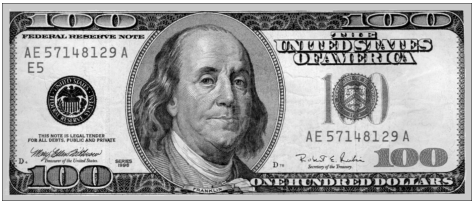
\includegraphics[width=\textwidth]{imagens_ft/dolar.png}
		\caption{Imagem original.}
		\label{fig:dolar_original1}
	\end{subfigure}
	\hfill
	\begin{subfigure}[b]{0.45\textwidth}
		\centering
		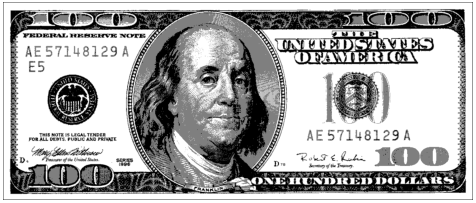
\includegraphics[width=\textwidth]{imagens_ft/limiar_dolar.png}
		\caption{Imagem limiarizada.}
		\label{fig:dolar_limiarizado}
	\end{subfigure}
	\caption{Aplicação da técnica de Limiarização.}
	\label{fig:limiar}
\end{figure}

Um caso particular da técnica de Limiarização é conhecido como Binarização, pois separa a imagem em dois tons de cinza: preto, representado pelo número $0$, e branco, representado pelo número $255$. É convencionado que o tom branco representa o objeto e o tom preto representa o fundo da imagem. A seguir, é definida a técnica de Binarização.

\begin{define}[\textit{Binarização}]
	Dada uma imagem $f(x,y)$ e $T \in [0,255]$, um número natural, o valor do limiar. A imagem $g(x,y)$ binarizada é dada como:
	\begin{equation}
		g(x,y) =
		\begin{cases}
			0, & \text{se} \; f(x,y) \geq T \\
			255, & \text{se} \; f(x,y)   <  T.
		\end{cases}
		\label{eq:binarizacao}
	\end{equation}
	\label{def:binarizacao}
\end{define}

A seguir é apresentado um exemplo aplicando a definição \ref{def:binarizacao}.

\begin{exemplo}
	Escolhendo como limiar $T = 127$, metade do caminho entre $0$ e $255$. Portanto, a equação \ref{eq:binarizacao} é escrita como: 
	\begin{equation}
		g(x,y) =
		\begin{cases}
			255, & \text{se} \; f(x,y) \geq 127 \\
			0, & \text{se} \; f(x,y)   <  127.
		\end{cases}
		\label{eq:exemplo_2}
	\end{equation}
	Seja a imagem $I(x,y) \subseteq \mathbb{N} \times \mathbb{N}$, expressa como:
	\begin{equation}
		I(x,y) = \begin{bmatrix}
			123 & 126 & 20 & 199 & 201 \\
			124 & 130 & 255 & 255 & 150 \\
			125 & 200 & 69 & 0 & 97 \\
			69 & 212 & 169 & 250 & 98 \\
			2 & 44 & 40 & 23 & 99
		\end{bmatrix}.
	\end{equation}
	Aplicando a equação \ref{eq:exemplo_2} é obtido $g(x,y)$, dada como: 
	\begin{equation}
		g(x,y) = \begin{bmatrix}
			0 &   0 &   0 & 255 & 255 \\
			0 & 255 & 255 & 255 & 255 \\
			0 & 255 &   0 &   0 &   0 \\
			0 & 255 & 255 & 255 &   0 \\
			0 &   0 &   0 &   0 &   0
		\end{bmatrix}.
	\end{equation}
\end{exemplo}

A figura \ref{fig:binario} apresenta uma imagem original e três imagens que foram binarizadas com valores de limiares diferentes. A figura \ref{fig:dolar_binario127} é uma binarização com $T = 127$, a figura \ref{fig:dolar_binario170} é uma binarização com $T = 170$ e a figura \ref{fig:dolar_binario87} é uma binarização com $T = 87$. 

\begin{figure}[h]
	\centering
	\begin{subfigure}[b]{0.45\textwidth}
		\centering
		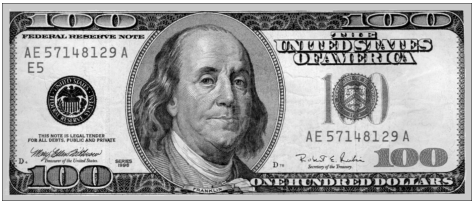
\includegraphics[width=\textwidth]{imagens_ft/dolar.png}
		\caption{Imagem original.}
		\label{fig:dolar_original}
	\end{subfigure}
	\hfill
	\begin{subfigure}[b]{0.45\textwidth}
		\centering
		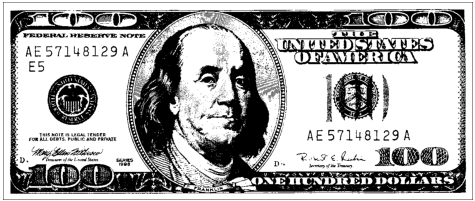
\includegraphics[width=\textwidth]{imagens_ft/binario_dolar.png}
		\caption{$T = 127$.}
		\label{fig:dolar_binario127}
	\end{subfigure}
	\hfill
	\begin{subfigure}[b]{0.45\textwidth}
		\centering
		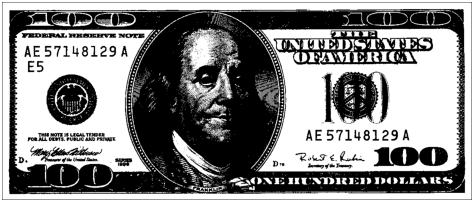
\includegraphics[width=\textwidth]{imagens_ft/binario170_dolar.png}
		\caption{$T = 170$.}
		\label{fig:dolar_binario170}
	\end{subfigure}
	\hfill
	\begin{subfigure}[b]{0.45\textwidth}
		\centering
		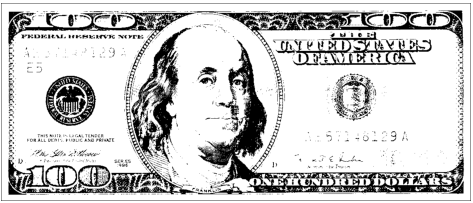
\includegraphics[width=\textwidth]{imagens_ft/binario87_dolar.png}
		\caption{$T = 87$.}
		\label{fig:dolar_binario87}
	\end{subfigure}
	\caption{Aplicação da técnica de Binarização.}
	\label{fig:binario}
\end{figure}

Observando a figura \ref{fig:binario}, nota-se que a escolha do valor de limiar é crucial para que o processo de segmentação baseada na Binarização produza bons resultados. Cabe ressaltar que a figura \ref{fig:dolar_original} não é uma imagem fácil de segmentar utilizando o segmentador Binarização, pois é uma imagem com muitas informações (texto, símbolos, letras e, claro, o ícone Benjamin Franklin) e essas informações são, em sua grande maioria, constituídas de muitos tons de cinza e não apenas de um tom de cinza, como aparenta.

Pelo exposto até aqui, o valor do limiar, $T$, é escolhido de forma arbitrária e subjetiva. Será que é possível determinar $T$ de maneira automática de modo que ele seja considerado o melhor para a imagem em estudo? Sim, é possível! Este método é apresentado a seguir.

\subsection{Limiarização Otsu}
%\label{subsection:imagens}

Agora, será apresentado o método de Limiarização Otsu \cite{otsu1979threshold}. Tal método é capaz de obter o melhor limiar para separar uma imagem em duas regiões apenas utilizando o Histograma desta imagem. A seguir, são expostos os passos matemáticos para o entendimento do funcionamento do método Otsu \cite{gonzalezprocessamento}. 

Tomemos o Histograma normalizado de uma imagem de dimensão $M \times N$. 

Após isso, escolhemos um limiar $k \in (0,255)$. Com isso, ficamos com duas classes: classe $C_1$, a qual é formada pelos pixels que estão no intervalo $[0,k]$, e classe $C_2$ formada pelos pixels que estão no intervalo $[k+1, L-1]$. A probabilidade de um pixel estar na classe $C_1$ é dada como,

\begin{equation}
	P_1(k) = \sum_{i=0}^{k} p_i
\end{equation}
e a probabilidade do pixel estar na classe $C_2$ é,

\begin{equation}
	P_2(k) = 1 - P_1(k).
\end{equation}

Agora, calcularemos a média das intensidades dos pixels que estão na classe $C_1$ e a média das intensidades dos pixels que compõe a classe $C_2$. A média de intensidade dos pixels da classe $C_1$ é calcula como 

\begin{equation}
	m_1(k) = \sum_{i=0}^{k} iP(i/C_1)
	\label{eq:otsu_m1}
\end{equation}
em que, o termo $P(i/C_1)$ é o teorema de Bayes\footnote{$P(A/B) = \dfrac{P(B/A)P(A)}{P(B)}$}. Substituindo a equação de Bayes na equação \ref{eq:otsu_m1} obtemos, 

\begin{equation}
	m_1(k) = \sum_{i=0}^{k} i \frac{P(C_1/i)P(i)}{P(C_1)}.
	\label{eq:otsu}
\end{equation}

Na equação \ref{eq:otsu}, é possível fazer algumas simplificações. $P(C_1/i) = 1$, pois estamos apenas trabalhando com valores possíveis para classe $C_1$. $P(i) = p_i$ e $P(C_1) = P_1(k)$. Portanto,

\begin{equation}
	m_1(k) = \sum_{i=0}^{k} i \frac{p_i}{P_1(k)}
	\label{eq:otsu_1}
\end{equation}

Para a média das intensidades dos pixels na classe $C_2$ o procedimento matemático é o mesmo, o qual resulta em  

\begin{equation}
	m_2(k) = \sum_{i=k+1}^{L-1} i \frac{p_i}{P_2(k)}.
	\label{eq:otsu_2}
\end{equation}

Sabemos que a intensidade média da imagem toda é 

\begin{equation}
	m_G = \sum_{i=0}^{L-1} ip_i.
\end{equation}

Podemos escrever $m_G$ em função de $m_1(k)$ e $m_2(k)$. Isolando os somatórios nas equações \ref{eq:otsu_1} e \ref{eq:otsu_2} obtemos,

\begin{equation}
	m_1(k)P_1(k) = \sum_{i=0}^{k} i p_i
	\label{eq:otsu_3}
\end{equation}
e

\begin{equation}
	m_2(k)P_2(k) = \sum_{i=k+1}^{L-1} i p_i.
	\label{eq:otsu_4}
\end{equation}

Somando as equações \ref{eq:otsu_3} e \ref{eq:otsu_4} temos 

\begin{equation}
	m_1(k)P_1(k) + m_2(k)P_2(k) = \sum_{i=0}^{k}ip_i + \sum_{i=k+1}^{L-1}ip_i = \sum_{i=0}^{L-1}ip_i = m_G,
\end{equation}
como queríamos escrever.

Para verificar a qualidade da segmentação com o limiar $k$ usamos a métrica de verificação 

\begin{equation}
	\eta = \frac{\sigma_B^2}{\sigma_G^2},
	\label{eq:otsu_metrica}
\end{equation}
em que, $\sigma_G^2$ é a \textit{variância global} definida como 

\begin{equation}
	\sigma_G^2 = \sum_{i=0}^{L-1} (i - m_G)^2 p_i
\end{equation}
e $\sigma_B^2$ é a \textit{variância entre classes} definida como 

\begin{equation}
	\sigma_B^2 = P_1(k)(m_1(k) - m_G)^2 + P_2(k)(m_2(k) - m_G)^2.
\end{equation}

O que queremos é maximizar a métrica de verificação, equação \ref{eq:otsu_metrica}. Na equação \ref{eq:otsu_metrica}, o termo $\sigma_G^2$ é uma constante, logo o termo que temos que maximizar é $\sigma_B^2$, ou seja, temos que encontrar o maior valor para a variância entre classes, $\sigma_B^2$. Matematicamente,

\begin{equation}
	\sigma_B^2(k*) = \max_{0 \geq k \geq L - 1} \sigma_B^2(k).
\end{equation}

Um bom jeito de realizar essa tarefa é calcular $\sigma_B^2$ para todos os valores de $k$ e selecionar o valor de $k$ que produz o maior valor. Caso o máximo exista para mais de um valor de $k$, calculamos a média dos valores de $k$ que atingiram o valor máximo.

A figura \ref{fig:otsu} mostra um comparativo entre a técnica de Binarização com limiar $T = 127$ e o método Otsu. O limiar encontrado pelo Otsu foi $T = 86$, para está imagem.

\begin{figure}[h]
	\centering
	\begin{subfigure}[b]{0.45\textwidth}
		\centering
		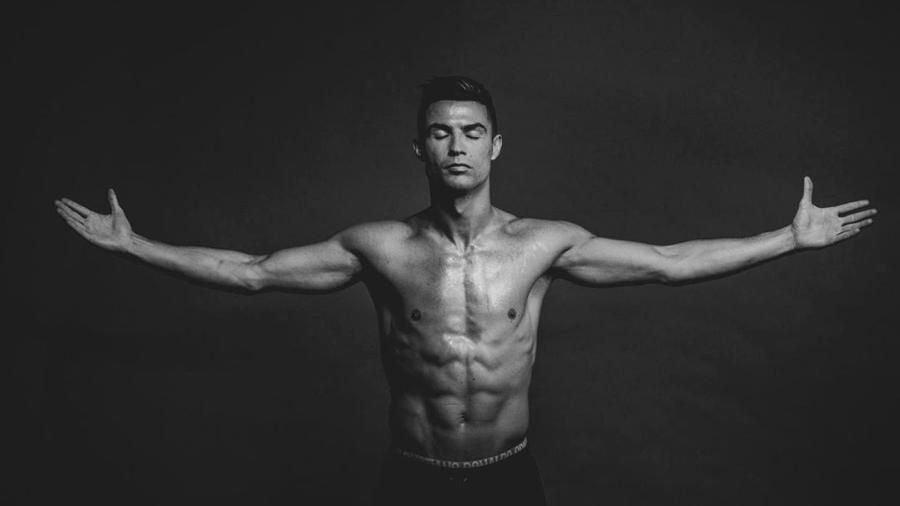
\includegraphics[width=0.85\textwidth]{imagens_ft/cr7.jpg}
		\caption{Imagem original.}
		\label{fig:otsu_original}
	\end{subfigure}
	\hfill
	\begin{subfigure}[b]{0.45\textwidth}
		\centering
		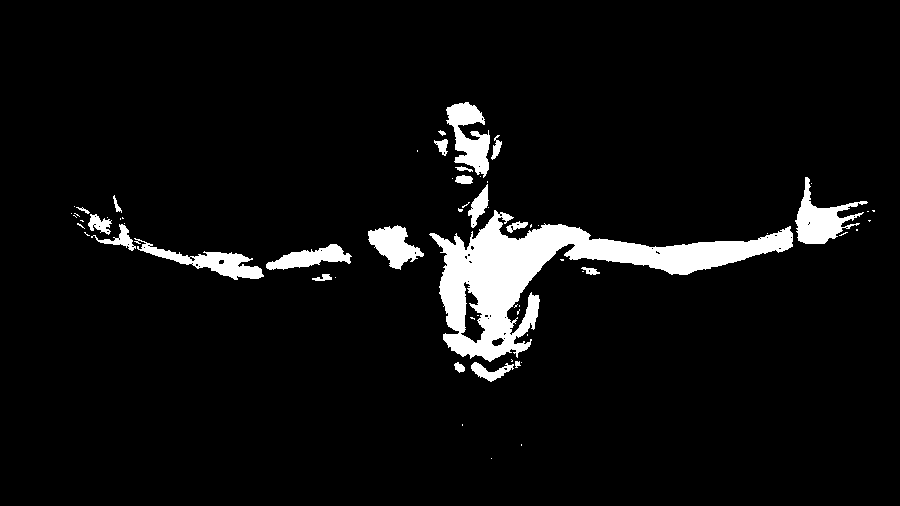
\includegraphics[width=0.85\textwidth]{imagens_ft/cr7_binario.png}
		\caption{Técnica Binarização, $T = 127$.}
		\label{fig:otsu_binario}
	\end{subfigure}
	\hfill
	\begin{subfigure}[b]{0.45\textwidth}
		\centering
		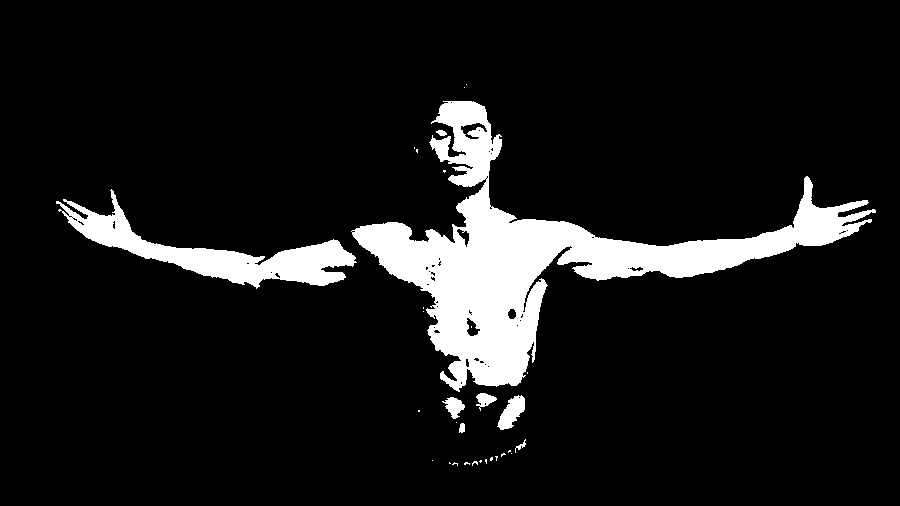
\includegraphics[width=0.85\textwidth]{imagens_ft/cr7_otsu.png}
		\caption{Técnica Otsu, $T = 86$.}
		\label{fig:otsu_aplicacao}
	\end{subfigure}
	\caption{Comparação da técnica Binarização com a técnica Otsu.}
	\label{fig:otsu}
\end{figure}

Até aqui, foram apresentados métodos de Limiarização conhecidos na literatura como Técnicas de Limiarização Global, pois o limiar calculado é utilizado para processar a imagem inteira. A partir de agora, estudaremos técnicas de Limiarização Local ou Adaptativo.

\subsection{Limiarização Local ou Adaptativo}

Suponha que queremos extrair o texto presente na figura \ref{fig:texto_original} utilizando técnicas de Processamento Digital de Imagens e conhecimentos de estatística. A primeira coisa que aplicamos é o método Otsu, visto que o mesmo retorna o melhor limiar para a imagem. O resultado da aplicação da técnica Otsu é mostrado na figura \ref{fig:texto_otsu}.

\begin{figure}[h]
	\centering
	\begin{subfigure}[b]{0.45\textwidth}
		\centering
		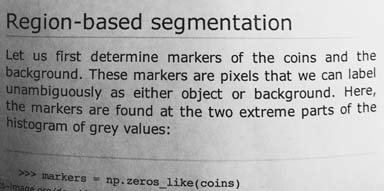
\includegraphics[width=0.9\textwidth]{imagens_ft/texto.png}
		\caption{Imagem original.}
		\label{fig:texto_original}
	\end{subfigure}
	\hfill
	\begin{subfigure}[b]{0.45\textwidth}
		\centering
		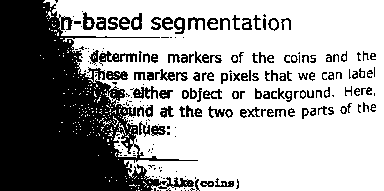
\includegraphics[width=0.9\textwidth]{imagens_ft/texto_otsu.png}
		\caption{Aplicação Otsu.}
		\label{fig:texto_otsu}
	\end{subfigure}
	\caption{Aplicação do método Otsu em uma imagem com diferença de iluminação.}
	\label{fig:texto}
\end{figure}

Observa-se na figura \ref{fig:texto_otsu} que a técnica Otsu não foi adequada para segmentar as palavras presentes na imagem, já que a imagem está borrada de preto, no canto esquerdo, atrapalhando a segmentação de algumas palavras. Esse borramento ocorre porque a figura \ref{fig:texto_original} apresenta uma diferença de iluminação, isto é, uma parte mais escura que a outra -- o lado esquerdo é mais escuro que o lado direito. 

O problema da iluminação observado na figura \ref{fig:texto_original} foi resolvido inicialmente por Niblack \cite{niblack1985introduction} e posteriormente por Sauvola \cite{sauvola2000adaptive}, o qual melhorou o método de Niblack. Com o tempo, muitos outros métodos foram criados, em sua grande maioria, para segmentação de documento Históricos. Tais métodos são chamados de Limiarização Variável, pois estes calculam o valor do limiar para cada região da imagem. Neste trabalho, chamaremos de Limiarização Adaptativa. A seguir são apresentados os métodos de Niblack, Sauvola e, também, o método Limiarização Adaptativa Gaussiana \cite{gonzalezprocessamento}. 

%As técnicas aqui apresentadas utilizam o processo de convolução, ou seja, é passado uma máscara pela imagem com tamanho pré-determinado pelo usuário. Para cada pixel da imagem é calculo uma medida estatística i a Limiarização é calculada para cada pixel. Por fim é aplicado a binarização, definição \ref{def:binarizacao}.

O método de Niblack utiliza a média, $m$, e o desvio padrão, $\sigma$, dos pixels contidos na janela deslizante para calcular o valor do limiar, $T$. O limiar $T$ é calculado como:

\begin{equation}
	T = m + k\sigma
\end{equation}
sendo $k$ um número, muita das vezes, entre zero e um. Por fim, é aplicada a definição \ref{def:binarizacao}. Um problema no método de Niblack é que ruídos presentes na imagem são apresentados na imagem segmentada.

O método de Sauvola é uma melhora do método de Niblack, isto é, o problema com os ruídos presentes no fundo da imagem foram corrigidos. O limiar $T$ é calculado como:

\begin{equation}
	T = m + mk\left(\frac{\sigma}{R} - 1\right)
\end{equation}
em que, $R$ e $k$ foram determinados por Sauvola através de experimentos práticos. Por fim, é aplicada a definição \ref{def:binarizacao}.

O método de Limiarização Adaptativa Gaussiana utiliza a média, $m$, e o desvio padrão, $\sigma$, dos pixels contidos na janela deslizante para calcular o valor do limiar, $T$. No entanto, primeiro é aplicado o filtro Gaussiano na janela deslizante. O limiar $T$ é calculado como:

\begin{equation}
	T = m + \sigma
\end{equation}
sendo, $m$ a média dos pixels depois de aplicado o filtro Gaussiano e $\sigma$ o desvio padrão dos pixels depois de aplicado o filtro Gaussiano. Por fim, é aplicada a definição \ref{def:binarizacao}.

Na figura \ref{fig:texto_limiarizacao} são mostrados os resultados das três técnicas de Limiarização apresentadas anteriormente. Para todas as técnicas foi utilizada uma janela de $25 \times 25$. Na técnica de Niblack, é utilizado $k = 0.8$. Na técnica de Sauvola é utilizado $k = 0.5$ e $R = 128$. 

\begin{figure}[h]
	\centering
	\begin{subfigure}[b]{0.45\textwidth}
		\centering
		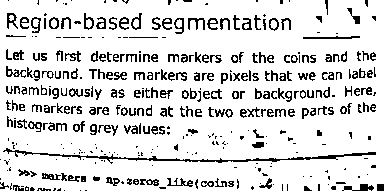
\includegraphics[width=0.85\textwidth]{imagens_ft/texto_niblack.png}
		\caption{Técnica Niblack.}
		\label{fig:texto_Niblack}
	\end{subfigure}
	\hfill
	\begin{subfigure}[b]{0.45\textwidth}
		\centering
		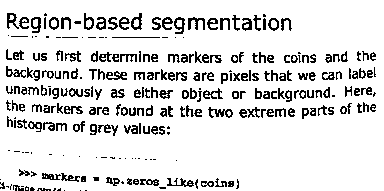
\includegraphics[width=0.85\textwidth]{imagens_ft/texto_sauvola.png}
		\caption{Técnica Sauvola.}
		\label{fig:texto_Sauvola}
	\end{subfigure}
	\hfill
	\begin{subfigure}[b]{0.45\textwidth}
		\centering
		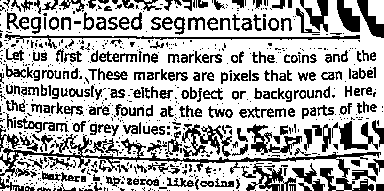
\includegraphics[width=0.85\textwidth]{imagens_ft/texto_gaussian.png}
		\caption{Técnica Limiarização Adaptativa Gaussiana.}
		\label{fig:texto_Gaussiana}
	\end{subfigure}
	\caption{Comparações das técnicas de Limiarização Adaptativa/Local.}
	\label{fig:texto_limiarizacao}
\end{figure}

\section{MORFOLOGIA MATEMÁTICA}

A Morfologia Matemática (MM) teve seu início na \textit{École Supérieure des Mines de Paris} com Georges Matheron e Jean Serra na década de 1960 \cite{faconmm}. Seu objetivo principal é extrair informações relativas à geometria e à topologia de um conjunto desconhecido de uma imagem utilizando-se dos conceitos matemáticos de teoria dos conjuntos \cite{pedrinischwartz}. 

Antes de apresentar as operações básicas da Morfologia Matemática, será apresentado o conceito de Elemento Estruturante de acordo com \cite{faconmm}. 

\begin{define}{(\textit{Elemento Estruturante})}
	É um conjunto definido e conhecido (forma e tamanho) que é comparado a partir de uma transformação ao conjunto desconhecido da imagem. 
\end{define}

Neste texto, o Elemento Estruturante será chamado de $B$. Algumas formas conhecidas de Elementos Estruturantes são: a cruz (\textit{Cr}), o disco (\textit{D}), o quadrado (\textit{Q}), a linha (\textit{L}) e a coluna (\textit{C}). Abaixo, são mostrados estes elementos. Neste trabalho, a origem do Elemento Estruturante é o \textit{pixel} central, o qual está destacado em vermelho.

\begin{equation}
	Cr =  \begin{bmatrix}
		0 & 1 & 0 \\
		1 & \textcolor{red}{1} & 1 \\
		0 & 1 & 0
	\end{bmatrix}, \;
	Q =  \begin{bmatrix}
		1 & 1 & 1 \\
		1 & \textcolor{red}{1} & 1 \\
		1 & 1 & 1
	\end{bmatrix}, \;
	C =  \begin{bmatrix}
		1 \\
		\textcolor{red}{1} \\
		1
	\end{bmatrix}, \;
	L =  \begin{bmatrix}
		1 & \textcolor{red}{1} & 1 
	\end{bmatrix}, \;
	D =  \begin{bmatrix}
		0 & 0 & 1 & 0 & 0 \\
		0 & 1 & 1 & 1 & 0 \\
		1 & 1 & \textcolor{red}{1} & 1 & 1 \\
		0 & 1 & 1 & 1 & 0 \\
		0 & 0 & 1 & 0 & 0 
	\end{bmatrix}
\end{equation}

Os tamanhos de $B$ podem ser alterados, por exemplo, o elemento \textit{Q} é um quadrado de lado $3$ mas podemos ter \textit{Q} com lado $2, 3, 4, 5, 6, ..., n \in \mathbb{N}$. Isso é válido para todos os Elementos Estruturantes.

A seguir será apresentado a Morfologia Matemática Binária e a Morfologia Matemática Cinza. Em cada seção será definido as operações básicas de Morfologia Matemática, Dilatação e Erosão, e as demais operações.

\subsection{Morfologia Matemática Binária}

As operações de Dilatação e Erosão serão definidas de acordo com \cite{pedrinischwartz} e \cite{haralick1987image}. As definições \ref{def:dilatacao_1} e \ref{def:erosao_1} podem ser encontradas em \cite{haralick1987image}. Já as definições \ref{def:dilatacao_2} e \ref{def:erosao_2} em \cite{pedrinischwartz}. As definições \ref{def:dilatacao_2} e \ref{def:erosao_2} são definidas como a adição de Minkowski e subtração de Minkowski, respectivamente.

\begin{define}[\textit{Dilatação}]
	Dados $A$ e $B$ subconjuntos do $\mathbb{Z}^2$. A dilatação de $A$ por $B$ é denotada por $A \oplus B$ e definida como
	
	\begin{equation}
		A \oplus B = \{c \in \mathbb{Z}^n | c = a + b \text{ para algum } a \in A \text{ e } b \in B\}.
	\end{equation}
	\label{def:dilatacao_1}
\end{define}

\begin{define}[\textit{Dilatação}]
	Seja $A$ e $B$ subconjuntos do $\mathbb{Z}^2$. A adição de Minkowski de $A$ com $B$, denotada por $A \oplus B$, é o seguinte conjunto:
	\begin{equation}
		A \oplus B = \bigcup_{b \in B} (A + b)
	\end{equation}
	\label{def:dilatacao_2}
\end{define}

Para elucidação da definição de Dilatação será feito um exemplo.

\begin{exemplo}
	Seja $A$ e $B$ subconjuntos do $\mathbb{Z}^2$, em que $\mathbb{Z}^2$ representa uma imagem binária. O conjunto $A$ é formado pelas coordenadas dos pixels da imagem que estão com valor 1 e o conjunto $B$ é formado pelas coordenadas dos pixels do Elemento Estruturante que estão com valor 1. Considere que as matrizes abaixo são uma imagem e um Elemento Estruturante, respectivamente.
	
	\begin{equation}
		I = \begin{bmatrix}
			0 & 1 & 0 & 0 & 0 \\
			0 & 1 & 0 & 0 & 0 \\
			0 & 1 & 1 & 0 & 0 \\
			1 & 0 & 0 & 0 & 0 \\
			0 & 0 & 0 & 0 & 0
		\end{bmatrix}, \; \; \; \; \; \; \; \; \; \; \; \; \; \; \; \; \; \; \; \;
		K = \begin{bmatrix}
			1 & 1
		\end{bmatrix}.
	\end{equation}
	
	\noindent Olhando para as matrizes, temos: $A = \{(0,1), (1,1), (2,1), (2,2), (3,0)\}$ e $B = \{(0,0), (0,1)\}$. A operação de dilatação vai ser um subconjunto de pontos do $\mathbb{Z}^2$ dado como,
	\begin{multline}
		A \oplus B = \{(0,1) + (0,0), \; (1,1) + (0,0), \; (2,1) + (0,0), \; (2,2) + (0,0), \; (3,0) + (0,0), \\ 
		\; (0,1) + (0,1), \; (1,1) + (0,1), \; (2,1) + (0,1), \; (2,2) + (0,1), \; (3,0) + (0,1)\}
	\end{multline}
	
	\noindent Realizando a soma de pares ordenados anterior temos que a dilatação da imagem $I$ pelo Elemento Estruturante $K$ é o conjunto, 
	\begin{equation}
		A \oplus B = \{(0,1), \; (1,1), \; (2,1), \; (2,2), \; (3,0), \; (0,2), \; (1,2), \; (2,2), \; (2,3), \; (3,1)\}.
	\end{equation}
	
	\noindent Dessa forma, a imagem dilatada é expressa como: 
	
	\begin{equation}
		I \oplus K = \begin{bmatrix}
			0 & 1 & 1 & 0 & 0\\
			0 & 1 & 1 & 0 & 0\\
			0 & 1 & 1 & 1 & 0\\
			1 & 1 & 0 & 0 & 0\\
			0 & 0 & 0 & 0 & 0
		\end{bmatrix}
	\end{equation}
\end{exemplo}

A figura \ref{fig:dilatacao} mostra na prática a operação de Dilatação.

\begin{figure}[h]
	\centering
	\begin{subfigure}[b]{0.4\textwidth}
		\centering
		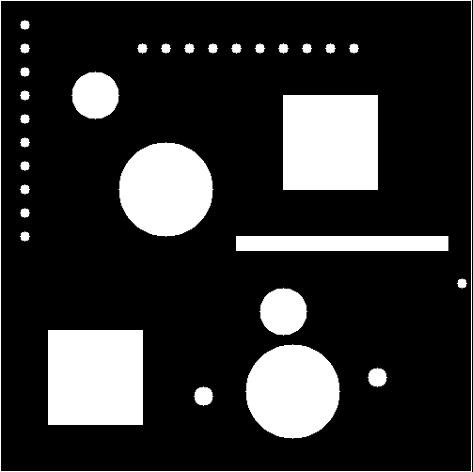
\includegraphics[width=0.75\textwidth]{imagens_ft/morfo_original.png}
		\caption{Imagem original.}
		\label{fig:original1}
	\end{subfigure}
	\hfill
	\begin{subfigure}[b]{0.4\textwidth}
		\centering
		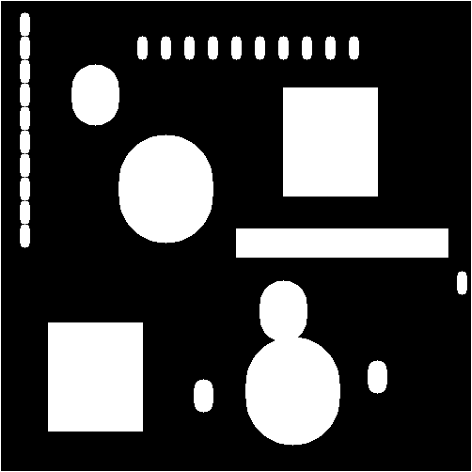
\includegraphics[width=0.75\textwidth]{imagens_ft/morfo_dil_coluna.png}
		\caption{Imagem dilatada com uma coluna.}
		\label{fig:dil_coluna}
	\end{subfigure}
	\hfill
	\begin{subfigure}[b]{0.4\textwidth}
		\centering
		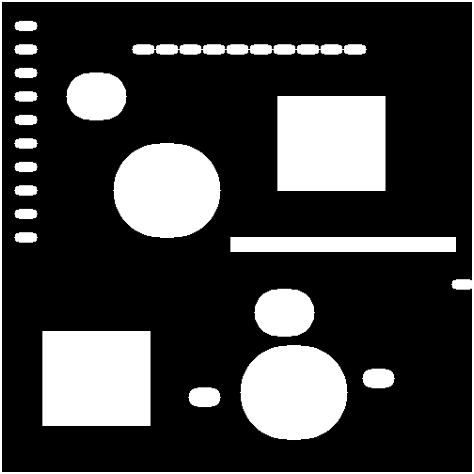
\includegraphics[width=0.75\textwidth]{imagens_ft/morfo_dil_linha.png}
		\caption{Imagem dilatada com uma linha.}
		\label{fig:dil_linha}
	\end{subfigure}
	\hfill
	\begin{subfigure}[b]{0.4\textwidth}
		\centering
		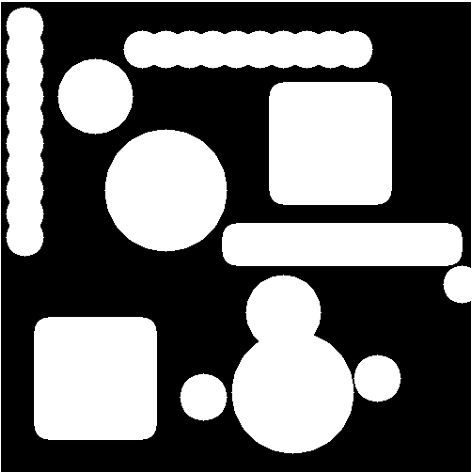
\includegraphics[width=0.75\textwidth]{imagens_ft/morfo_dil_disco.png}
		\caption{Imagem dilatada com um disco.}
		\label{fig:dil_disco}
	\end{subfigure}
	\caption{Exemplos de imagens dilatadas.}
	\label{fig:dilatacao}
\end{figure}

Analisando a figura \ref{fig:dilatacao}, nota-se que os objetos contidos na imagem alteram sua forma de acordo com o formato do Elementos Estruturante. Verifica-se que na figura \ref{fig:dil_coluna} os objetos na imagem ficaram mais alongados na vertical enquanto na figura \ref{fig:dil_linha} os objetos foram alongados na horizontal. Isso acontece pois na figura \ref{fig:dil_coluna} foi utilizado o Elemento Estruturante coluna e na figura \ref{fig:dil_linha} foi utilizado o Elemento Estruturante linha, ambos de tamanho $15$. Já na figura \ref{fig:dil_disco}, foi utilizado o Elemento Estruturante disco de raio $15$, o qual deixou os objetos que constituem a imagem arredondados. Portanto, quando aplicado a técnica de \textit{Dilatação} pode concluir que,

\begin{itemize}
	\item[$\rightarrow$] o tamanho dos objetos são aumentados;
	\item[$\rightarrow$] os pequenos buracos são preenchidos; 
	\item[$\rightarrow$] pode ocorrer a conexão dos objetos próximos; e
	\item[$\rightarrow$] a deformação dos objetos depende do Elemento Estruturante.
\end{itemize}

\begin{define}[\textit{Erosão}]
	Dados $A$ e $B$ subconjuntos do $\mathbb{Z}^2$. A erosão de $A$ por $B$ é denotada por $A \ominus B$ e definida como
	\begin{equation}
		A \ominus B = \{x \in \mathbb{Z}^2 | x + b \text{ para cada } b \in B\}.
	\end{equation}
	\label{def:erosao_1}
\end{define}

\begin{define}[\textit{Erosão}]
	Sejam $A$ e $B$ subconjuntos do $\mathbb{Z}^2$. A subtração de Minkowski de $A$ com $B$, denotada por $A \ominus B$, é o seguinte conjunto: 
	\begin{equation}
		A \ominus B = \bigcap_{b \in B} (A - b)
	\end{equation}
	\label{def:erosao_2}
\end{define}

Para compreensão da definição de Erosão será feito o seguinte exemplo.

\begin{exemplo}
	Seja $A$ e $B$ subconjuntos do $\mathbb{Z}^2$, em que $\mathbb{Z}^2$ representa uma imagem binária. O conjunto $A$ é formado pelas coordenadas dos pixels da imagem que estão com valor 1 e o conjunto $B$ é formado pelas coordenadas dos pixels do Elemento Estruturante que estão com valor 1. Considere que as matrizes abaixo são uma imagem e um Elemento Estruturante, respectivamente.
	
	\begin{equation}
		I = \begin{bmatrix}
			0 & 0 & 0 & 0 & 0 & 0 & 0 \\
			0 & 1 & 1 & 1 & 0 & 0 & 0 \\
			0 & 0 & 0 & 1 & 1 & 0 & 0 \\
			0 & 1 & 1 & 1 & 1 & 0 & 0 \\
			0 & 0 & 1 & 1 & 1 & 0 & 0 \\
			0 & 0 & 0 & 0 & 0 & 0 & 0 \\
			0 & 0 & 0 & 0 & 0 & 0 & 0
		\end{bmatrix},  \; \; \; \; \; \; \; \; \; \; \; \; \; \; \; \; \; \; \; \;
		K = \begin{bmatrix}
			1 & 1 \\
			1 & 1
		\end{bmatrix}.
	\end{equation}
	
	\noindent Olhando para as matrizes $I$ e $K$, é obtido os conjuntos $A$ e $B$:
	\begin{equation}
		A = \{(1,1), \; (1,3), \; (2,1), \; (2,3), \; (2,4), \; (3,1), \; (3,2), \; (3,3), \; (3,4), \; (4,2), \; (4,3), \; (4,4)\}, \text{ e }
	\end{equation} 
	\begin{equation}
		B = \{(0,0), \; (0,1), \; (1,0), \; (1,1)\}.
	\end{equation} 
	
	\noindent A Erosão é a intersecção dos conjuntos, $A - (0,0)$, $A - (0,1)$, $A - (1,0)$ e $A - (1,1)$. A seguir, é obtido os conjuntos $A - (0,0)$ e $A - (0,1)$.
	
	\begin{multline}
		A - (0,0) = \{(1,1) - (0,0), \; (1,3) - (0,0), \; (2,1) - (0,0), \; (2,3) - (0,0), \\ \; (2,4) - (0,0), \; (3,1) - (0,0), \; (3,2) - (0,0), \; (3,3) - (0,0), \\ \; (3,4) - (0,0), \; (4,2) - (0,0), \; (4,3) - (0,0), \; (4,4) - (0,0)\}.
	\end{multline}
	Então, 
	\begin{equation}
		A - (0,0) = \{(1,1), \; (1,3), \; (2,1), \; (2,3), \; (2,4), \; (3,1), \; (3,2), \; (3,3), \; (3,4), \; (4,2), \; (4,3), \; (4,4)\}
	\end{equation}
	Fazendo a mesma operação para o ponto $(0,1)$.
	\begin{multline}
		A - (0,1) = \{(1,1) - (0,1), \; (1,3) - (0,1), \; (2,1) - (0,1), \; (2,3) - (0,1), \\ \; (2,4) - (0,1), \; (3,1) - (0,1), \; (3,2) - (0,1), \; (3,3) - (0,1), \\ \; (3,4) - (0,1), \; (4,2) - (0,1), \; (4,3) - (0,1), \; (4,4) - (0,1)\}.
	\end{multline}
	Então, 
	\begin{equation}
		A - (0,1) = \{(1,0), \; (1,2), \; (2,0), \; (2,2), \; (2,3), \; (3,0), \; (3,1), \; (3,2), \; (3,3), \; (4,1), \; (4,2), \; (4,3)\}
	\end{equation}
	
	\noindent Analogamente para os pontos $(1,0)$ e $(1,1)$ é obtido mais dois conjuntos $A - (1,0)$ e $A - (1,1)$. Por fim, aplicando a definição \ref{def:erosao_2},
	
	\begin{align}
		I \ominus K & = (A - (0,0)) \cap (A - (1,0)) \cap (A - (0,1)) \cap (A - (1,1)) \\
		& = \{(3,2), \; (3,3), \; (2,3)\}.
	\end{align}
	
	\noindent Dessa forma, a imagem erodida é dada como: 
	
	\begin{equation}
		I \oplus K = \begin{bmatrix}
			0 & 0 & 0 & 0 & 0 & 0 & 0 \\
			0 & 0 & 0 & 0 & 0 & 0 & 0 \\
			0 & 0 & 0 & 1 & 0 & 0 & 0 \\
			0 & 0 & 1 & 1 & 0 & 0 & 0 \\
			0 & 0 & 0 & 0 & 0 & 0 & 0 \\
			0 & 0 & 0 & 0 & 0 & 0 & 0 \\
			0 & 0 & 0 & 0 & 0 & 0 & 0 
		\end{bmatrix}
	\end{equation}
\end{exemplo}

A figura \ref{fig:erosao} mostra visualmente a operação de Erosão. Observando a figura \ref{fig:erosao} conclui-se que os objetos variam suas formas de acordo com o Elemento Estruturante. Nas figuras \ref{fig:ero_coluna}, \ref{fig:ero_linha} e \ref{fig:ero_disco} é observado que alguns objetos sumiram, pois estes são menores que o Elemento Estruturante. Também é notado que os objetos diminuíram seus tamanhos. Portanto, quando aplicamos a \textit{Erosão} pode concluir que:

\begin{itemize}
	\item[$\rightarrow$] o tamanho dos objetos são diminuídos; 
	\item[$\rightarrow$] ocorre a eliminação dos elementos de tamanho inferior ao tamanho do Elemento Estruturante;
	\item[$\rightarrow$] há um aumento dos buracos; e
	\item[$\rightarrow$] acontece a separação de objetos próximos;
\end{itemize}

\begin{figure}[h]
	\centering
	\begin{subfigure}[b]{0.4\textwidth}
		\centering
		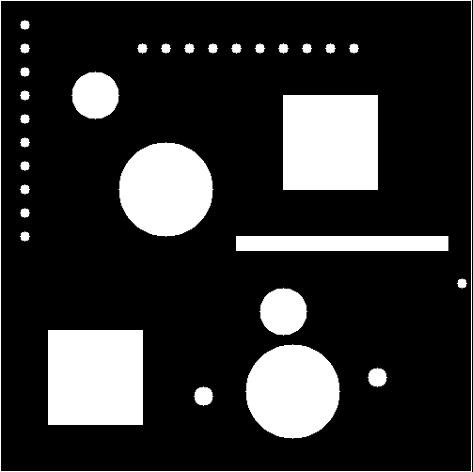
\includegraphics[width=0.75\textwidth]{imagens_ft/morfo_original.png}
		\caption{Imagem original.}
		\label{fig:original2}
	\end{subfigure}
	\hfill
	\begin{subfigure}[b]{0.4\textwidth}
		\centering
		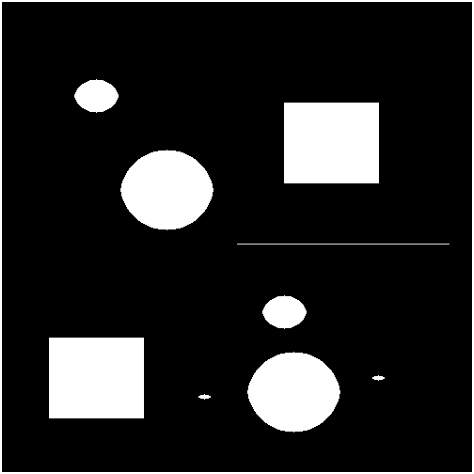
\includegraphics[width=0.75\textwidth]{imagens_ft/morfo_ero_coluna.png}
		\caption{Imagem erodida com uma coluna.}
		\label{fig:ero_coluna}
	\end{subfigure}
	\hfill
	\begin{subfigure}[b]{0.4\textwidth}
		\centering
		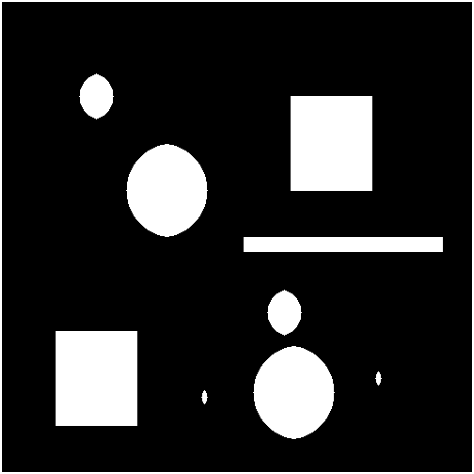
\includegraphics[width=0.75\textwidth]{imagens_ft/morfo_ero_linha.png}
		\caption{Imagem erodida com uma linha.}
		\label{fig:ero_linha}
	\end{subfigure}
	\hfill
	\begin{subfigure}[b]{0.4\textwidth}
		\centering
		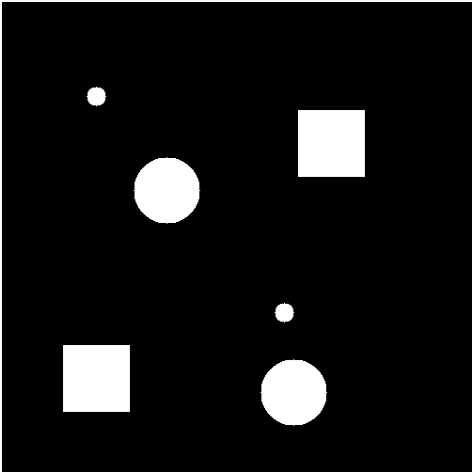
\includegraphics[width=0.75\textwidth]{imagens_ft/morfo_ero_disco.png}
		\caption{Imagem erodida com um disco.}
		\label{fig:ero_disco}
	\end{subfigure}
	\caption{Exemplos de imagens erodidas.}
	\label{fig:erosao}
\end{figure}

A seguir, será apresentado uma propriedade da Dilatação e da Erosão. Em \cite{haralick1987image}, são apresentadas todas as propriedades que a Dilatação e a Erosão possuem e, também, suas respectivas demonstrações.

\begin{propriedade}
	Seja A uma imagem e B um Elemento Estruturante, ambos subconjuntos do $\mathbb{Z}^2$. As operações de Dilatação e Erosão são duais com relação à complementação e à reflexão, isto é,
	\begin{enumerate}
		\item[(a)] $(A \oplus B)^c  = A^c \ominus B'$
		\item[(b)] $(A \ominus B)^c = A^c \oplus B' $,
	\end{enumerate}
	em que $A^c$ representa o complementar de $A$ e $B'$ denota a reflexão de B, isto é, $B' = \{ -b | b \in B\}$.
\end{propriedade}

Uma aplicação imediata das operações de Dilatação e Erosão é a Extração de Bordas. A seguir é definido tal operação.

\begin{define}[\textit{Extração de Borda}]
	Seja $A$ uma imagem e $B$ um Elemento Estruturante, ambos subconjuntos do $\mathbb{Z}^2$. Seja $X$ um elemento de $A$. A borda do elemento $X$, denotada por $E(X)$, é obtida como
	\begin{equation}
		E(X) = A - (A \ominus B).
		\label{eq:grad_interno}
	\end{equation}
	A equação \ref{eq:grad_interno} é chamada de \textit{Gradiente Interno}. Outra forma de obter a borda do elemento $X$ é
	\begin{equation}
		E(X) = (A \oplus B) - A.
		\label{eq:grad_externo}
	\end{equation}
	A equação \ref{eq:grad_externo} é chamada de \textit{Gradiente Externo}. Somando as equações \ref{eq:grad_interno} e \ref{eq:grad_externo} obtemos o \textit{Gradiente Morfológico}, mostrado na equação \ref{eq:grad_morfologico}.
	\begin{equation}
		E(X) = (A \oplus B) - (A \ominus B).
		\label{eq:grad_morfologico}
	\end{equation}
\end{define}

Exemplificando a definição de Extração de Borda.

\begin{exemplo}
	\label{ex:morfo_borda}
	Seja $A$ e $B$ subconjuntos do $\mathbb{Z}^2$, em que $\mathbb{Z}^2$ representa uma imagem binária. O conjunto $A$ é formado pelas coordenadas dos pixels da imagem que estão com valor 1 e o conjunto $B$ é formado pelas coordenadas dos pixels do Elemento Estruturante que estão com valor 1. Considere que as matrizes abaixo são uma imagem e um Elemento Estruturante, respectivamente.
	\begin{displaymath}
		I = \begin{bmatrix}
			0 & 0 & 0 & 0 & 0 & 0 & 0 & 0 & 0 & 0 \\
			0 & 1 & 1 & 1 & 1 & 1 & 1 & 1 & 1 & 0 \\
			0 & 1 & 1 & 1 & 1 & 1 & 1 & 1 & 1 & 0 \\
			0 & 1 & 1 & 1 & 1 & 1 & 1 & 1 & 1 & 0 \\
			0 & 1 & 1 & 1 & 0 & 0 & 1 & 1 & 1 & 0 \\
			0 & 1 & 1 & 1 & 0 & 0 & 1 & 1 & 1 & 0 \\
			0 & 0 & 0 & 0 & 0 & 0 & 0 & 0 & 0 & 0 \\ 
		\end{bmatrix}, \; \; \; \; \; \; \; \; \; \; \; \; \; \;
		K = \begin{bmatrix}
			1 & 1 & 1 \\
			1 & 1 & 1 \\
			1 & 1 & 1
		\end{bmatrix}.
	\end{displaymath}
	\noindent Assim, para $I$ e $K$,
	\begin{multline}
		A = \{(1,1), \; (1,2), \; (1,3), \; (1,4), \; (1,5), \; (1,6), \; (1,7), \; (1,8), \; (2,1), \; (2,2), \\ \; (2,3), \; (2,4), \; (2,5), \; (2,6), \; (2,7), \; (2,8), \; (3,1), \; (3,2), \; (3,3), \; (3,4), \\ \; (3,5), \; (3,6), \; (3,7), \; (3,8), \; (4,1), \; (4,2), \; (4,3), \; (4,6), \; (4,7), \; (4,8), \\
		(5,1), \; (5,2), \; (5,3), \; (5,6), \; (5,7), \; (5,8) \}
	\end{multline}
	\begin{equation}
		B = \{(0,0), \; (0,1), \; (0,2), \; (1,0), \; (1,1), \; (1,2), \; (2,0), \; (2,1), \; (2,2)\}.
	\end{equation}
	\noindent Para determinar a borda, aplicamos a equação \ref{eq:grad_interno}. A seguir, é realizado dois passos para encontrar o conjunto $A \ominus B$.
	\begin{multline}
		A - (0,0)= \{(1,1), \; (1,2), \; (1,3), \; (1,4), \; (1,5), \; (1,6), \; (1,7), \; (1,8), \; (2,1), \; (2,2), \\ \; (2,3), \; (2,4), \; (2,5), \; (2,6), \; (2,7), \; (2,8), \; (3,1), \; (3,2), \; (3,3), \; (3,4), \\ \; (3,5), \; (3,6), \; (3,7), \; (3,8), \; (4,1), \; (4,2), \; (4,3), \; (4,6), \; (4,7), \; (4,8), \\
		(5,1), \; (5,2), \; (5,3), \; (5,6), \; (5,7), \; (5,8) \}
	\end{multline}
	\begin{multline}
		A - (0,1)= \{(1,0), \; (1,1), \; (1,2), \; (1,3), \; (1,4), \; (1,5), \; (1,6), \; (1,7), \; (2,0), \; (2,1), \\ \; (2,2), \; (2,3), \; (2,4), \; (2,5), \; (2,6), \; (2,7), \; (3,0), \; (3,1), \; (3,2), \; (3,3), \\ \; (3,4), \; (3,5), \; (3,6), \; (3,7), \; (4,0), \; (4,1), \; (4,2), \; (4,5), \; (4,6), \; (4,7), \\
		(5,0), \; (5,), \; (5,2), \; (5,5), \; (5,6), \; (5,7) \}
	\end{multline}
	\noindent Analogamente para os pontos $(0,2)$, $(1,0)$, $(1,1)$, $(1,2)$, $(2,0)$, $(2,1)$ e $(2,2)$ obtemos mais $7$ conjuntos. Aplicando a definição \ref{def:erosao_2},
	\begin{multline}
		A \ominus B = (A - (0,0)) \cap (A - (0,1)) \cap (A - (0,2)) \cap (A - (1,0)) \\ \cap (A - (1,1)) \cap (A - (1,2)) \cap (A - (2,0)) \cap (A - (2,1)) \cap (A - (2,2)).
	\end{multline}
	\begin{multline}
		A \ominus B = \{(2,2), \; (3,2), \; (4,2), \; (4,3), \; (4,4), \; (4,5), \; (4,6), \\ \; (4,7), \; (4,8), \; (4,9), \; (3,6), \; (3,7), \; (3,8), \; (2,6), \; (2,7), \; (2,8)\}.
	\end{multline}
	\noindent Fazendo a diferença de conjuntos entre o conjunto $A$ e o conjunto $A \ominus B$, encontramos a borda do objeto, 
	\begin{multline}
		A - (A \ominus B) = \{(1,1), \; (2,1), \; (3,1), \; (4,1), \; (5,1), \; (5,2), \; (5,3), \; (5,4), \\ \; (5,5), \; (5,6), \; (5,7), \; (5,8), \; (5,9), \; (5,10), \; (4,10), \; (3,10), \\ \; (3,9), \; (2,9), \; (1,9), \; (1,8), \; (1,7), \; (1,6), \; (1,5), \; (2,5), \\ \; (3,5), \; (3,4), \; (3,3), \; (2,3), \; (1,3), \; (1,2), \; (1,1)\}.
	\end{multline}
	\noindent Dessa forma, o Gradiente Interno é dado como: 
	\begin{displaymath}
		I - (I \ominus K) = \begin{bmatrix}
			0 & 0 & 0 & 0 & 0 & 0 & 0 & 0 & 0 & 0 \\
			0 & 1 & 1 & 1 & 1 & 1 & 1 & 1 & 1 & 0 \\
			0 & 1 & 0 & 0 & 0 & 0 & 0 & 0 & 1 & 0 \\
			0 & 1 & 0 & 1 & 1 & 1 & 1 & 0 & 1 & 0 \\
			0 & 1 & 0 & 1 & 0 & 0 & 1 & 0 & 1 & 0 \\
			0 & 1 & 1 & 1 & 0 & 0 & 1 & 1 & 1 & 0 \\
			0 & 0 & 0 & 0 & 0 & 0 & 0 & 0 & 0 & 0 
		\end{bmatrix}.
	\end{displaymath}
\end{exemplo}

A figura \ref{fig:gradiente}, mostra visualmente a técnica de extração de bordas.

\begin{figure}[h]
	\centering
	\begin{subfigure}[b]{0.4\textwidth}
		\centering
		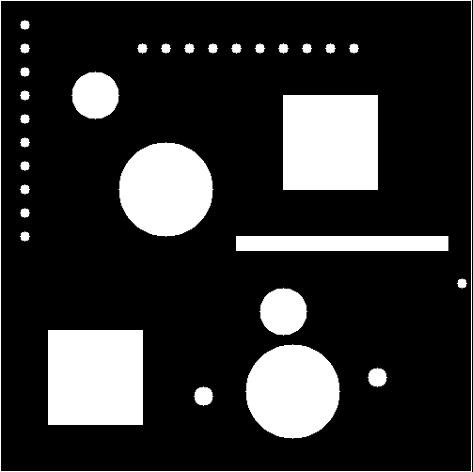
\includegraphics[width=0.75\textwidth]{imagens_ft/morfo_original.png}
		\caption{Imagem original.}
		\label{fig:original3}
	\end{subfigure}
	\hfill
	\begin{subfigure}[b]{0.4\textwidth}
		\centering
		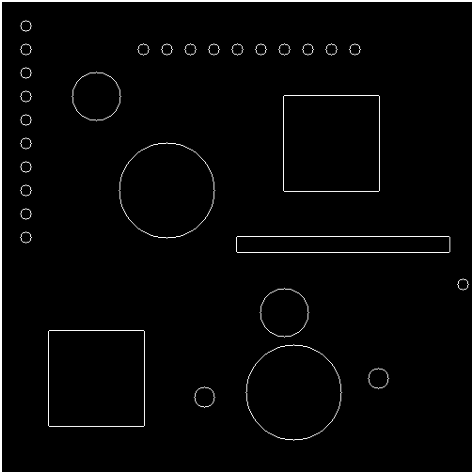
\includegraphics[width=0.75\textwidth]{imagens_ft/morfo_grad_ex.png}
		\caption{Gradiente Externo.}
		\label{fig:grad_externo}
	\end{subfigure}
	\hfill
	\begin{subfigure}[b]{0.4\textwidth}
		\centering
		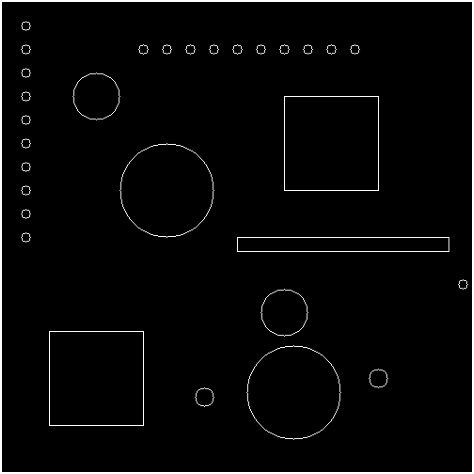
\includegraphics[width=0.75\textwidth]{imagens_ft/morfo_grad_in.png}
		\caption{Gradiente Interno.}
		\label{fig:grad_in}
	\end{subfigure}
	\hfill
	\begin{subfigure}[b]{0.4\textwidth}
		\centering
		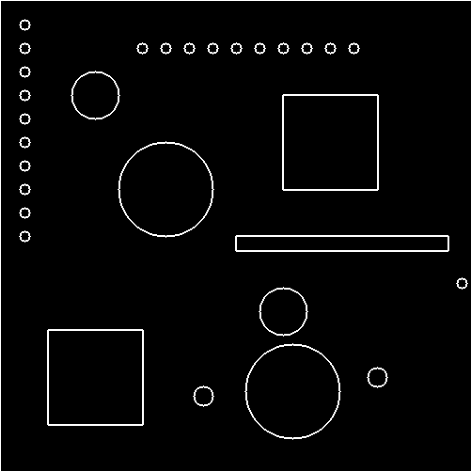
\includegraphics[width=0.75\textwidth]{imagens_ft/morfo_grad_mor.png}
		\caption{Gradiente Morfológico}
		\label{fig:grad_mor}
	\end{subfigure}
	\caption{Exemplos da extração da borda com Morfologia Matemática.}
	\label{fig:gradiente}
\end{figure}

A partir da \textit{Dilatação} e da \textit{Erosão} é possível determinar as demais operações que compõem a Morfologia Matemática. Neste trabalho, apresentaremos as operações de Abertura, Fechamento e Reconstrução. 

\begin{define}[\textit{Abertura}]
	A Abertura da imagem $A$ pelo Elemento Estruturante $B$ é denotada por $A \circ B$ e é definida como 
	\begin{equation}
		A \circ B = (A \ominus B) \oplus B.
	\end{equation}
\end{define}

\begin{define}[\textit{Fechamento}]
	O Fechamento da imagem $A$ pelo Elemento Estruturante $B$ é denotado por $A \bullet B$ e definido como
	\begin{equation}
		A \bullet B = (A \oplus B) \ominus B.
	\end{equation}
\end{define}

%%%%%%%%%%%%%% MORFOLOGIA MATEMÁTICA EM CINZA. 

\subsection{Morfologia Matemática Cinza}

As operações de Dilatação e Erosão serão definidas de acordo com \cite{gonzalezprocessamento} e \cite{pedrinischwartz}.

\begin{define}[\textit{Dilatação}]
	A dilatação de uma imagem monocromática $f$ por um elemento estruturante $B$ é definida como
	\begin{equation}
		[f \oplus B](x,y) = \max_{(s,t) \in B}\{f(x+s,y+t)\}.
	\end{equation}
\end{define}

% exemplo dilatação
\begin{exemplo}
	
	Seja $f$ uma imagem digital em tons de cinza e $B$ o Elemento Estruturante Quadrado $3 \times 3$.
	
	\begin{equation}
		f = \begin{bmatrix}
			20 & 23 & 26 & 28 & 32 & 25 & 25 & 17 \\
			17 & 19 & 19 & 35 & 28 & 34 & 33 & 28 \\
			34 & 36 & 27 & 33 & 37 & 44 & 40 & 41 \\
			32 & 27 & 18 & 16 & 21 & 26 & 28 & 32 \\
			34 & 27 & 25 & 23 & 24 & 35 & 37 & 29 
		\end{bmatrix}, \; \; \; \; \; \; \; \; \; \; \; \; \; \; \; \; \; \; \; \;
		B = \begin{bmatrix}
			1 & 1 & 1 \\
			1 & 1 & 1 \\
			1 & 1 & 1 
		\end{bmatrix}.
	\end{equation}
	
	A dilatação de $f$ pelo elemento $B$ é realizada deslocando o elemento estruturante sobre a imagem e tomando o máximo entre os valores que estão dentro do Elemento Estruturante. Por exemplo, supondo que a origem do Elemento Estruturante esteja sobre o \textit{pixel} de intensidade 19 (linha 2, coluna 2) o resultado da dilatação é o máximo entre $\{20, 23, 26, 17, 19, 19, 34, 36, 27\}$, ou seja, 36. O resultado da dilatação é mostrado na equação \ref{eq:matriz_dilatacao_cinza}.
	
	\begin{equation}
		[f \oplus B] = \begin{bmatrix}
			23 & 26 & 35 & 35 & 35 & 34 & 34 & 33 \\
			36 & 36 & 36 & 37 & 37 & 44 & 44 & 41 \\
			36 & 36 & 36 & 37 & 37 & 44 & 44 & 41 \\
			36 & 36 & 36 & 37 & 44 & 44 & 44 & 41 \\
			34 & 34 & 27 & 25 & 35 & 37 & 37 & 37
		\end{bmatrix}.
		\label{eq:matriz_dilatacao_cinza}
	\end{equation}
\end{exemplo}

A figura \ref{fig:dilatacao_cinza} mostra na prática a operação de Dilatação em imagens monocromáticas.

\begin{figure}[h]
	\centering
	\begin{subfigure}[b]{0.45\textwidth}
		\centering
		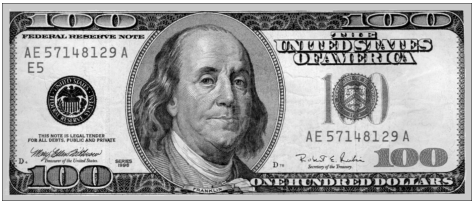
\includegraphics[width=\textwidth]{imagens_ft/dolar.png}
		\caption{Imagem original.}
		\label{fig:dolar_mm_d}
	\end{subfigure}
	\hfill
	\begin{subfigure}[b]{0.45\textwidth}
		\centering
		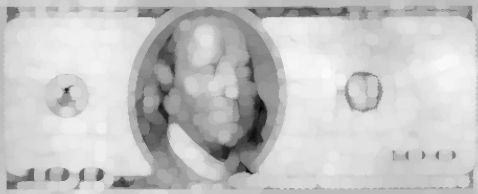
\includegraphics[width=\textwidth]{imagens_ft/dolar_dilatacao.png}
		\caption{Imagem dilatada utilizando o E.E. disco.}
		\label{fig:dolar_mm_dilatacao}
	\end{subfigure}
	\caption{Exemplo de imagem dilatada.}
	\label{fig:dilatacao_cinza}
\end{figure}

Observando a figura \ref{fig:dilatacao_cinza}, é notado que a figura \ref{fig:dolar_mm_d} ficou totalmente deformada após aplicação do operador morfológico dilatação. Na figura \ref{fig:dolar_mm_dilatacao}, nota-se que a as escritas que existem na nota de 100 dólares está praticamente apagada e, também, a cara de Benjamin Franklin fica irreconhecível. Analisando a figura \ref{fig:dolar_mm_dilatacao} conclui-se que a dilatação em nível de cinza tem as seguintes propriedades: 

\begin{itemize}
	\item[$\rightarrow$] clarear a imagem;
	\item[$\rightarrow$] aumentar os padrões claros da imagem;
	\item[$\rightarrow$] juntar os locais claros da imagem; 
	\item[$\rightarrow$] reduzir e as vezes eliminar os vales, isto é, os pontos escuros da imagem; 
	\item[$\rightarrow$] separar os vales próximos. 
\end{itemize}

\begin{define}[\textit{Erosão}]
	A erosão de uma imagem monocromática $f$ por um elemento estruturante $B$ é definida como
	\begin{equation}
		[f \ominus B](x,y) = \min_{(s,t) \in B}\{f(x+s,y+t)\}.
	\end{equation}
\end{define}

% exemplo erosão
\begin{exemplo} 
	
	Seja $f$ uma imagem digital em tons de cinza e $B$ o Elemento Estruturante Quadrado $3 \times 3$.
	
	\begin{equation}
		f = \begin{bmatrix}
			20 & 23 & 26 & 28 & 32 & 25 & 25 & 17 \\
			17 & 19 & 19 & 35 & 28 & 34 & 33 & 28 \\
			34 & 36 & 27 & 33 & 37 & 44 & 40 & 41 \\
			32 & 27 & 18 & 16 & 21 & 26 & 28 & 32 \\
			34 & 27 & 25 & 23 & 24 & 35 & 37 & 29 
		\end{bmatrix}, \; \; \; \; \; \; \; \; \; \; \; \; \; \; \; \; \; \; \; \;
		B = \begin{bmatrix}
			1 & 1 & 1 \\
			1 & 1 & 1 \\
			1 & 1 & 1 
		\end{bmatrix}.
	\end{equation}
	
	A erosão de $f$ pelo elemento $B$ é realizada deslocando o elemento estruturante sobre a imagem e tomando o mínimo entre os valores que estão dentro do Elemento Estruturante. Por exemplo, supondo que a origem do Elemento Estruturante esteja sobre o \textit{pixel} de intensidade 16 (linha 4, coluna 4) o resultado da erosão é o mínimo entre $\{27, 33, 37, 18, 16, 21, 25, 23, 24\}$, ou seja, 16. O resultado da erosão é mostrado na equação \ref{eq:matriz_erosao_cinza}.
	
	
	\begin{equation}
		[f \ominus B] = \begin{bmatrix}
			17 & 17 & 19 & 19 & 25 & 25 & 17 & 17 \\
			17 & 17 & 19 & 19 & 25 & 25 & 17 & 17 \\
			17 & 17 & 16 & 16 & 16 & 21 & 26 & 28 \\
			27 & 18 & 16 & 16 & 16 & 21 & 26 & 28 \\
			27 & 18 & 16 & 16 & 16 & 21 & 26 & 28 
		\end{bmatrix}.
		\label{eq:matriz_erosao_cinza}
	\end{equation}
\end{exemplo}

A figura \ref{fig:erosao_cinza} mostra na prática a operação de Erosão em imagens monocromáticas.

\begin{figure}[h]
	\centering
	\begin{subfigure}[b]{0.45\textwidth}
		\centering
		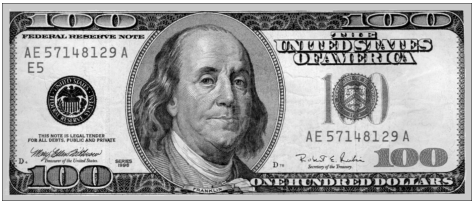
\includegraphics[width=\textwidth]{imagens_ft/dolar.png}
		\caption{Imagem original.}
		\label{fig:dolar_mm_e}
	\end{subfigure}
	\hfill
	\begin{subfigure}[b]{0.45\textwidth}
		\centering
		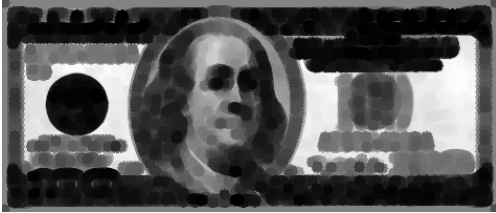
\includegraphics[width=\textwidth]{imagens_ft/dolar_erosao.png}
		\caption{Imagem erodida utilizando o E.E. disco.}
		\label{fig:dolar_mm_erosao}
	\end{subfigure}
	\caption{Exemplo de imagem erodida.}
	\label{fig:erosao_cinza}
\end{figure}

Observando a figura \ref{fig:erosao_cinza}, é notado que a figura \ref{fig:dolar_mm_e} ficou totalmente deformada após aplicação do operador morfológico erosão. Na figura \ref{fig:dolar_mm_erosao}, nota-se que as escritas que existem na nota de 100 dólares está praticamente tampadas pela cor preto e cinza. Também, a cara de Benjamin Franklin está deformada. Analisando a figura \ref{fig:dolar_mm_erosao} conclui-se que a erosão em nível de cinza tem as seguintes propriedades: 

% erosão
\begin{itemize}
	\item[$\rightarrow$] escurecer a imagem;
	\item[$\rightarrow$] aumentar os padrões escuros da imagem;
	\item[$\rightarrow$] juntar os locais escuros da imagem;
	\item[$\rightarrow$] reduzir e as vezes eliminar os picos, isto é, os pontos claros da imagem;
	\item[$\rightarrow$] separar picos próximos.
\end{itemize}

Definidas as operações de Dilatação e de Erosão é possível determinar as demais operações que há na Morfologia Matemática em tons de cinza. Neste trabalho, será apresentado as operações de Abertura, Fechamento, Dilatação Geodésica, Erosão Geodésica, Reconstrução, Abertura por Reconstrução e Fechamento por Reconstrução.

As operações Dilatação Geodésica, Erosão Geodésica, Reconstrução, Abertura por Reconstrução e Fechamento por Reconstrução são definidas, pois são necessárias para implementar os Filtro Sequencia Alternado (\textit{Alternating Sequence Filter} – ASF).

\begin{define}[\textit{Abertura}]
	A abertura da imagem $f$ pelo elemento estruturante $B$ é dada por
	\begin{equation}
		f \circ B = (f \ominus B) \oplus B
	\end{equation}
\end{define}

\begin{define}[\textit{Fechamento}]
	O fechamento da imagem $f$ pelo elemento estruturante $B$ é dado por
	\begin{equation}
		f \bullet B = (f \oplus B) \ominus B
	\end{equation}
\end{define}

\begin{define}[\textit{Dilatação Geodésica}]
	Seja $f$ e $g$ imagens em níveis de cinza de mesmo tamanho tal que $f \leq g$ e $B$ um elemento estruturante. $f$ é chamada de \textit{marcador} e $g$ é chamada de \textit{máscara}. A dilatação geodésica de tamanho 1 é definida como
	\begin{equation}
		D_{g}^{(1)}(f) = (f \oplus B) \wedge g, 
	\end{equation}
	em que $\wedge$ é o operador mínimo pontual. A dilatação geodésica de tamanho $n$ de $f$ em relação a $g$ é definida como
	\begin{equation}
		D_{g}^{(n)}(f) = D_{g}^{(1)}[D_{g}^{(n-1)}(f)]
	\end{equation}
	com $D_{g}^{(0)}(f) = f$.
\end{define}

\begin{define}[\textit{Erosão Geodésica}]
	Seja $f$ e $g$ imagens em níveis de cinza de mesmo tamanho tal que $f \leq g$ e $B$ um elemento estruturante. $f$ é chamada de \textit{marcador} e $g$ é chamada de \textit{máscara}. A erosão geodésica de tamanho 1 é definida como
	\begin{equation}
		E_{g}^{(1)}(f) = (f \ominus B) \vee g
	\end{equation}
	em que $\vee$ é o operador máximo pontual. A erosão geodésica de tamanho $n$ de $f$ em relação a $g$ é definida como
	\begin{equation}
		E_{g}^{(n)}(f) = E_{g}^{(1)}[E_{g}^{(n-1)}(f)]
	\end{equation}
	com $E_{g}^{(0)}(f) = f$.
\end{define}

\begin{define}[\textit{Reconstrução Morfológica por Dilatação}]
	Seja $f$ e $g$ imagens em tons de cinza, sendo $f$ a imagem marcador e $g$ a imagem máscara. A reconstrução morfológica por dilatação é definida como a dilatação geodésica de $f$ em relação a $g$ até atingir a estabilidade, isto é, $D_{g}^{(k)}(f) = D_{g}^{(k+1)}(f)$ 
	\begin{equation}
		R_{g}^{D}(f) = D_{g}^{(k)}(f).
	\end{equation}    
\end{define}

\begin{define}[\textit{Reconstrução Morfológica por Erosão}]
	Seja $f$ e $g$ imagens em tons de cinza, sendo $f$ a imagem marcador e $g$ a imagem máscara. A reconstrução morfológica por dilatação é definida como a dilatação geodésica de $f$ em relação a $g$ até atingir a estabilidade, isto é, $E_{g}^{(k)}(f) = E_{g}^{(k+1)}(f)$
	\begin{equation}
		R_{g}^{E}(f) = E_{g}^{(k)}(f).
	\end{equation}
\end{define}

\begin{define}[\textit{Abertura por Reconstrução}]
	A abertura por reconstrução de tamanho $n$ de uma imagem $f$ é definida como a reconstrução por dilatação de $f$ a partir da erosão de tamanho $n$ de $f$, matematicamente,
	\begin{equation}
		O^{(n)}_{R}(f) = R^{D}_{f}[(f \ominus nB)] = f \circ_D B,
	\end{equation}
	em que $(f \ominus nb)$ denota $n$ erosões de $f$ por $B$. 
\end{define}

\begin{define}[\textit{Fechamento por Reconstrução}]
	O fechamento por reconstrução de tamanho $n$ de uma imagem $f$ é definida como a reconstrução por erosão de $f$ a partir da dilatação de tamanho $n$ de $f$, matematicamente,
	\begin{equation}
		C^{(n)}_{R}(f) = R^{E}_{f}[(f \oplus nB)] = f \bullet_D B,
	\end{equation}
	em que $(f \oplus nB)$ denota $n$ dilatações de $f$ por $B$.
\end{define}

A seguir, será definido o Filtro Sequencia Alternado (\textit{Alternating Sequence Filter} – ASF). Tal definição pode ser encontrada em \cite{dougherty2003hands}.

\begin{define}[\textit{Filtro Sequencial Alternado fechamento -- abertura }]
	Seja $f$ uma imagem em tons de cinza e $B$ um elemento estruturante. O Filtro Sequência Alternado fechamento -- abertura de estágio $n$, $ASF^{n}_{fa,B,D}(f)$, é definido matematicamente como
	
	\begin{equation}
		ASF^{n}_{fa,B,D}(f) = (((((f \bullet_D B) \circ_D B) \bullet_D 2B) \circ_D 2B) \dots \bullet_D nB) \circ_D nB,
	\end{equation}
	em que $f \bullet_D B$ e $f \circ_D B$ são, respectivamente, \textit{Fechamento por Reconstrução} e \textit{Abertura por Reconstrução}.
\end{define}

\begin{define}[\textit{Filtro Sequencial Alternado abertura -- fechamento }]
	Seja $f$ uma imagem em tons de cinza e $B$ um elemento estruturante. O Filtro Sequência Alternado abertura -- fechamento de estágio $n$, $ASF^{n}_{af,B,D}(f)$, é definido matematicamente como
	
	\begin{equation}
		ASF^{n}_{af,B,D}(f) = (((((f \circ_D B) \bullet_D B) \circ_D 2B) \bullet_D 2B) \dots \circ_D nB) \bullet_D nB. 
	\end{equation}
	em que $f \circ_D B$ e $f \bullet_D B$ são, respectivamente, \textit{Abertura por Reconstrução} e \textit{Fechamento por Reconstrução}.
\end{define}

\section{YOLO}

A rede neural convolucional YOLO (\textit{You Only Look Once}) é uma técnica de Visão Computacional que ganhou muita popularidade nos últimos anos, pelo seu desempenho na detecção de objetos em tempo real ser muito superior quando comparado com as técnicas existentes, R-CNN e \textit{Fast} R-CNN \cite{yolo, yolo2}. 

Publicada em 2016 por Joseph Redmon\footnote{\url{https://pjreddie.com/}, página pessoal de Joseph Redmon.} no CVPR \cite{yolo} a YOLO é capaz de processar, isto é, identificar objetos em uma imagem em apenas 0,05 segundos enquanto as técnicas R-CNN e \textit{Fast} R-CNN levam aproximadamente 0,5 segundos. Por esta velocidade de processamento, a YOLO tem sido utilizada em várias áreas do conhecimento. Destacam-se áreas como: robótica, agricultura, medicina e segurança no trânsito. Em robótica há um grande número de aplicações na área de veículos autônomos, principalmente na parte de detecção de obstáculos. Na agricultura, a YOLO é muito utilizada para a classificação de culturas e para a localização de pragas e doenças em lavouras. Na área médica, a YOLO está sendo utilizada para detecção de câncer levando a uma melhor precisão do diagnóstico e processos de tratamento mais eficientes. Por fim, a YOLO tem sido utilizada no sistemas de trânsito contribuindo para o desenvolvimento de sistemas de transporte inteligentes e soluções de gerenciamento de tráfego\footnote{\url{https://www.youtube.com/watch?v=Cgxsv1riJhI&t=1s} é possível ver Joseph Redmon demonstrando a YoLo em tempo real.}. Além dessa performance, o seu código é livre para uso. Para o funcionamento desta técnica, Joseph Redmon desenvolveu uma arquitetura de rede neural profunda chamada de \textit{Darknet}\footnote{\url{https://github.com/pjreddie/darknet}} \cite{yolo}.

A baixo é explicado de forma bem básica o funcionamento da rede neural YOLO \cite{yolo1}.

\begin{itemize}
	\item A imagem de entrada é dividida em uma grade $S \times S$.
	
	\item Cada célula da grade prevê $B$ caixas delimitadoras e, também, a pontuação de confiança. A YOLO utiliza recursos de toda a imagem para prever as caixas delimitadoras. Dessa forma, todas as caixas delimitadoras são determinadas simultaneamente em uma imagem. A pontuação de confiança mostra se há um objeto e, também, quão precisa ela acha que a caixa prevê. A confiança é definida como 
	
	\begin{equation}
		Pr(Object) \ast IOU^{truth}_{pred}.
	\end{equation} 
	
	Se não existe objeto naquela célula, pontuações de confiança é igual a zero. Caso contrário, a pontuação de confiança deve ser igual à IOU entre a caixa prevista e o \textit{ground truth}.
	
	\item Cada caixa delimitadora gera 5 previsões: $x$, $y$, $w$, $h$, e confiança. $(x, y)$ representam o centro da caixa em relação aos limites da célula da grade, $w$ a largura e $h$ a altura. Por fim, a confiança representa o IOU entre o caixa prevista e qualquer caixa \textit{ground truth}.
	
	\item Para avaliar o desempenho do modelo a YOLO utiliza as métrica \textit{Average Precision} (AP) e a técnica \textit{Non-Maximum Suppression} (NMS). A métrica \textit{Average Precision} avalia o desempenho de modelos de detecção de objetos. Já a técnica \textit{Non-Maximum Suppression} é utilizada no pós-processamento de algoritmos de detecção de objetos para reduzir o número de caixas delimitadoras sobrepostas e melhorar a qualidade geral da detecção.
\end{itemize} 

A arquitetura de rede da YOLO é inspirada no GoogLeNet. Tal rede é composta por 24 camadas convolucionais seguidas por 2 camadas totalmente conectadas. Uma das diferença entre a GoogLeNet e a YOLO é que a GoogLeNet utiliza módulos iniciais e a YOLO utiliza camadas de redução 1 × 1 seguidas por camadas convolucionais 3 × 3 \cite{yolo1}. A figura \ref{fig:arquitetura_YOLO} ilustra a arquitetura de rede YOLO.

\begin{figure}[H]
	\centering
	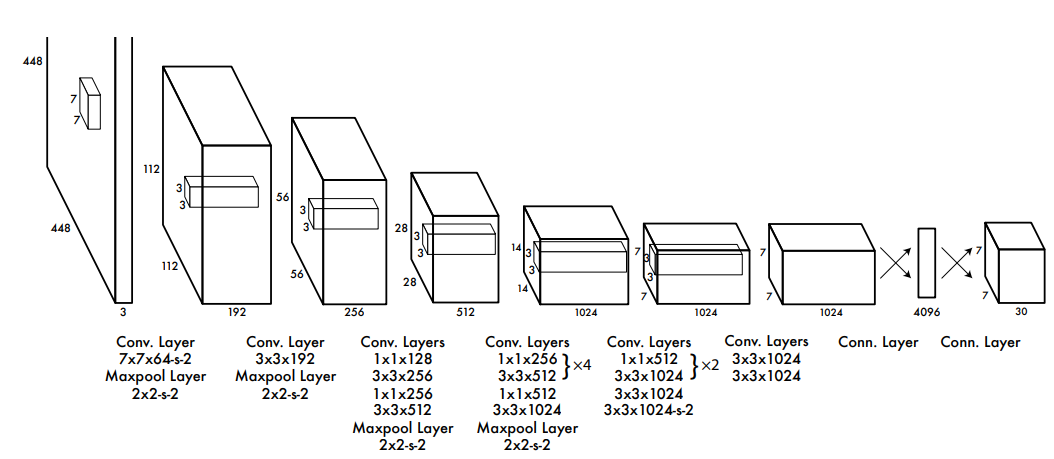
\includegraphics[width = 16cm, height = 7cm]{imagens_ft/arq_yolo.png}
	\caption{Arquitetura YOLO. \cite{yolo1}}
	\label{fig:arquitetura_YOLO}
\end{figure}

Em \cite{yolo1} é possível encontrar a arquitetura das redes neurais convolucional YOLO utilizada neste trabalho.

\section{PROPRIEDADES GEOMÉTRICAS}

A seguir, são definidos os conceitos de perímetro, área e circularidade para um objeto em uma imagem digital. Tais definições podem ser encontradas em \cite{pedrinischwartz}.

\begin{define}[\textit{Perímetro}]
	O perímetro representa o comprimento da borda de um objeto.
	\label{def:perimetro}
\end{define}

Uma aproximação para o cálculo de perímetro pode ser obtida pela contagem dos pixels ao longo da borda do objeto na imagem. 

\begin{define}[\textit{Área}]
	A área pode ser expressa como o número de pixels que compreende o objeto ou a região de interesse.
	\label{def:area}
\end{define}

Em uma imagem binária, por exemplo, um objeto que pertence a essa imagem tem sua área e perímetro calculada como a soma de todos os pixels que estão na cor branca, valor $255$ ou $1$, quando normalizado.

\begin{define}[\textit{Circularidade}]
	A circularidade de uma região é definida como
	\begin{equation}
		C = \frac{P^2}{A},
		\label{eq:circularidade}
	\end{equation}
	em que $A$ e $P$ são a área e o perímetro da região, respectivamente, medidos em unidades de pixel.
\end{define}

Essas três propriedades geométricas são invariante quanto às operações de translação e rotação. A circularidade é, também, invariante à escala.

\begin{exemplo}
	
	Seja $A$ uma imagem binária definida como
	
	\begin{equation}
		A = \begin{bmatrix}
			0 & 0 & 0 & 0 & 0 & 0 & 0 & \textcolor{blue}{1} & 0 & 0 \\
			0 & \textcolor{red}{1} & \textcolor{red}{1} & \textcolor{red}{1} & 0 & 0 & \textcolor{blue}{1} & \textcolor{blue}{1} & \textcolor{blue}{1} & 0 \\
			0 & \textcolor{red}{1} & \textcolor{red}{1} & \textcolor{red}{1} & 0 & \textcolor{blue}{1} & \textcolor{blue}{1} & \textcolor{blue}{1} & \textcolor{blue}{1} & \textcolor{blue}{1} \\
			0 & \textcolor{red}{1} & \textcolor{red}{1} & \textcolor{red}{1} & 0 & 0 & \textcolor{blue}{1} & \textcolor{blue}{1} & \textcolor{blue}{1} & 0 \\
			0 & 0 & 0 & 0 & 0 & 0 & 0 & \textcolor{blue}{1} & 0 & 0 \\
			0 & 0 & 0 & 0 & 0 & 0 & 0 & 0 & 0 & 0 \\
			0 & 0 & 0 & 0 & 0 & 0 & 0 & 0 & 0 & 0 \\ 
		\end{bmatrix}.
	\end{equation}
	
	É notado que existe dois elementos na imagem um quadrado, em vermelho, e uma circunferência, em azul. Calculemos a área de ambos objetos: $Aq = 9$ e $Ac = 13$. Agora calculamos o perímetro: $Pq = 8$ e $Pc = 8$. Como a imagem é binária, a área é calculado contando quantos pixel da cor branca há no objeto e o perímetro é calculado contando quantos pixel da cor branca há na borda. Por fim, obtemos a circularidade do quadrado ($Cq$) e do círculo ($Cc$).
	
	\begin{equation}
		Cq = \frac{8^2}{9} = 7,11
	\end{equation}
	
	\begin{equation}
		Cc = \frac{8^2}{13} = 4,92
	\end{equation}
	
\end{exemplo}

\section{APRENDIZAGEM DE MÁQUINA}

\subsection{$k$--NN}

O \textit{k--Nearest Neighbors} ($k$--NN) ou $k$--Vizinhos Mais Próximos é um algoritmo de aprendizado de máquina muito utilizado para problemas de classificação, pois seu funcionamento é simples e traz bons resultados em diversas aplicações \cite{knn2}. Para realizar a classificação de amostras desconhecidas, esse método utiliza cálculo de distância entre dois pontos no $\mathbb{R}^n$. As métricas de distâncias mais utilizadas são:

\begin{itemize}
	\item Distância Euclidiana, matematicamente expressa por:
	
	\begin{equation}
		D_e(x,y) = \sqrt{\sum_{i=1}^{n} (x_i - y_i)^2}.
		\label{eq:euclidiana}
	\end{equation}
	
	\item Distância Manhattan ou distância do Táxi, matematicamente expressa por:
	
	\begin{equation}
		D_m(x,y) = \sum_{i=1}^{n} |(x_1 - y_1)|.
		\label{eq:manhattan}
	\end{equation}
	
	\item Distância Minkowski, matematicamente expressa por:
	
	\begin{equation}
		D_M(x,y) = \sqrt[q]{\sum_{i=1}^{n} |x_i - y_i|^q}, \text{em que $q \in \mathbb{N}$}.
		\label{eq:minkowski}
	\end{equation}
\end{itemize}

A distância de Minkowski é a generalização das distâncias Euclidiana e Manhattan. Tomando $q = 1$, é obtido a distância de Manhattan e quando tomamos $q = 2$ é obtido a distância Euclidiana. Para as equações anteriores $x = (x_1, x_2, \dots, x_n)$ e $y = (y_1, y_2, \dots, y_n)$ são dois pontos do $\mathbb{R}^n$.

Com uma das distâncias escolhidas anteriormente, é calculado a distância da amostra com rótulo desconhecida para todas as amostras que possuem rótulo conhecidos. Após isso, é escolhido os $k$'s menores valores de distâncias. O rótulo do elemento com rótulo desconhecido é obtido pela maioria dentre os rótulos desses $k$'s elementos selecionados. Com isso, é notado que $k$ é o principal parâmetro do algoritmo e deve ser escolhido com cuidado. Muita das vezes, o valor de $k$ é um valor pequeno e ímpar para minimizar o risco de empate em classificação binária. Escolhas comuns são algo como 3, 5 e 7. Porém, pode-se fazer testes de classificação variando valores de $k$, para definir o melhor valor \cite{knn1}. 

A desvantagem desse método é o custo computacional, pois para cada novo exemplo, deve calcular a distância para todos os outros exemplos, além de ser sensível a ruídos nos dados. Vale lembrar que o algoritmo utiliza variáveis numéricas que devem ser, de preferência, normalizadas \cite{knn3}.

\subsection{SVM}

O \textit{Support Vector Machine} (SVM) é uma técnica bastante utilizada em problemas de classificação binária. Esta técnica de aprendizagem de máquina tem por objetivo encontrar um hiperplano em um espaço $n$-dimensional que possa classificar os dados. Desenvolvido utilizando as teorias de Vapnik–Chervonenkis \cite{vapnik1995nature} no final dos anos 90, foi proposta como uma solução não-linear para tarefas de classificação e regressão. Para problemas binários, a separação pode ser realizada por diversos hiperplanos. O SVM tenta encontrar um hiperplano ótimo, tentando maximizar a margem de ambos os pontos de entrada de cada classe \cite{svm1, svm2}. Esses hiperplanos são considerados limites de decisão, que são a base para a classificação do conjunto de dados. Dependendo do número de entradas, o hiperplano pode ter $n$ dimensões. A figura \ref{fig:svm} mostra um hiperplano ótimo separando dois conjuntos.

\begin{figure}[H]
	\centering
	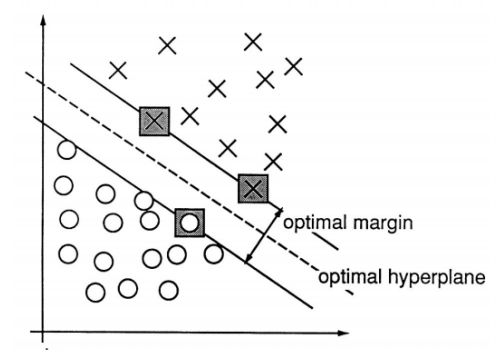
\includegraphics[width = 7.5cm, height = 5.3cm]{imagens_ft/svm.png}
	\caption{Representação de solução do SVM. \cite{vapnik1995nature}}
	\label{fig:svm}
\end{figure}

Por fim, os vetores de suporte são os dados que estão mais próximos do hiperplano, que influenciam na orientação e posição do mesmo. Qualquer alteração nesses vetores de suporte causa uma mudança na posição do hiperplano, já que são eles que ajudam a construir o SVM.

\section{TEXTURA}

A textura pode ser definida como um conjunto de características estatísticas ou outras propriedades locais da imagem, que sejam constantes, com pouca variação ou aproximadamente periódicas \cite{gonzalezprocessamento}. A textura é uma importante característica para a análise de imagens em diferentes aplicações. Atualmente, a extração de textura em imagens tem sido utilizada na resolução de problemas de classificação nas áreas de medicina, biometria, segurança, análise de imagens de satélites, entre outras. As abordagens para extrair descritores de textura são: Estatística, Estrutural e Espectral \cite{gonzalezprocessamento}. Neste trabalho será utilizado o descritor estrutural \textit{Local Phase Quantization} (LPQ).

\subsection{Local Phase Quantization (LPQ)}

Os desfoques presentes nas imagens podem limitar a análise das informações de textura. Algoritmos que removem esses desfoques são computacionalmente custosos e podem introduzir novos artefatos, portanto, são desejados algoritmos que possam analisar texturas de maneira robusta.

Ojansivu e Heikkila \cite{ojansivu2008blur} propuseram um descritor de textura insensível ao desfoque, baseado na fase quantizada da transformada discreta de Fourier, denominado \textit{Local Phase Quantization} (LPQ). A informação da fase local de uma imagem de tamanho $N \times N$ é dada pela Transformada de Fourier de Curto Prazo na Equação \ref{eq:STFT}, sendo $\Phi_{u_{i}}$ definida pela Equação \ref{eq:freq2d}, em que $r = (m - 1)/2$ e $u_i$ é um vetor de frequência 2D

\begin{equation}
	\hat{f}_{u_{i}}(x) = (f \times \Phi_{u_{i}})x,
	\label{eq:STFT}
\end{equation} 

\begin{equation}
	\Phi_{u_{i}} = e^{-j2\pi u^{T}_{i} y} |y \in \mathbb{Z}^2||y||\infty \leq r.
	\label{eq:freq2d}
\end{equation} 

Apenas quatro coeficientes complexos são considerados no LPQ, que correspondem à frequência 2D $u_1 = [a,0]^T$, $u_2 = [0,a]^T$, $u_3 = [a,a]^T$ , $u_4 = [a,-a]^T$, sendo $a = 1/m$. O STFT (Equação \ref{eq:STFT}) é expresso usando a notação vetor descrito em \ref{eq:vetorNotacao}. Com $w_u$ sendo o vetor base STFT em uma frequência $u$ e $f(x)$, um vetor de tamanho $m^2$ contendo os valores dos pixels da imagem no $m$ $\times$ $m $ vizinhança de $x$.

\begin{equation}
	\hat{f}_{u_{i}}(x) = w^{T}_{u_{i}}f(x)
	\label{eq:vetorNotacao}
\end{equation}

Sendo $F = [f(x_1),f(x_2)...,f(x_{n^2})]$ denotado como uma matriz $m^2 \times N^2$ contendo a vizinhança de todos os pixels da imagem e $w = [w_R,w_I]^T$, em que $w_R = Re[w_{u_1},w_{u_2},w_{u_3},w_{u_4}]$ e $w_I = Im[w_{u_1} ,w_{u_2},w_{u_3},w_{u_4}]$. $Re[]$ e $Im[]$ representam, respectivamente, as partes real e imaginária de um número complexo e a matriz de transformação $(8 \times N^2)$ é dada por $\hat{F} = wF$ .

Ojansivu e Heikkila \cite{ojansivu2008blur} assumem que a função $f(x)$ de uma imagem é o resultado do processo de Markov de primeira ordem, em que o coeficiente de correlação entre dois pixels $x_i$ e $x_j$ está exponencialmente relacionado à sua $L^2$ distância. O vetor $f$ é definido por uma matriz de covariância de tamanho $m^2 \times m^2$ conforme a Equação \ref{eq:covariância}, e a matriz de covariância dos coeficientes de Fourier pode ser obtida por $D = wC{w}^T$. Contanto que $D$ não seja uma matriz diagonal, os coeficientes são correlacionados e podem se tornar não correlacionados através de $E = V^T\hat{F}$, onde $V$ é uma matriz ortogonal derivada da decomposição de valor singular ( SVD) de uma matriz D, que é $D' = V^TDV$.

\begin{equation}
	C_{i,j} = \sigma^{||x_{i} - x_{j}||}
	\label{eq:covariancia}
\end{equation}

Os coeficientes são quantizados utilizando a equação \ref{eq:quantizar}, na qual $e_{ij}$ são componentes de $E$. Os coeficientes são representados como valores inteiros entre 0 e 255 utilizando o código binário obtido da equação \ref{eq:binarizar}.

Por fim, um histograma desses valores inteiros de todas as posições das imagens é usado para formar um vetor de características de 256 dimensões usado para classificação. 

\begin{equation}
	q_{i,j} = \left\{ 
	\begin{array}{ll}
		1, & \mbox{if $e_{i,j} \geq 0$},\\
		0, & \mbox{otherwise}.
	\end{array} \right.
	\label{eq:quantizar}
\end{equation}

\begin{equation}
	b_{j} = \sum_{i=0}^{7} q_{i,j}2^j
	\label{eq:binarizar}
\end{equation}

\subsection{Granulometria}

Suponha que queremos saber quantos objetos de tamanho $t_1$, $t_2$, $\dots$, $t_n$ existe na imagem \ref{fig:granulometria}. Uma ferramenta que permite saber a quantidade de objetos de tamanhos distintos é a Granulometria. A Granulometria pode ser facilmente entendida realizando analogia com o processo de peneiramento de objetos, pois o processo de peneiramento é separar elementos de acordo com o tamanho. O processo de Granulometria é a realização de vários peneiramento alterando todas as vezes o tamanho da malha da peneira. Dessa forma é possível determinar a quantidade de objetos de acordo com seu tamanho.

\begin{figure}[H]
	\centering
	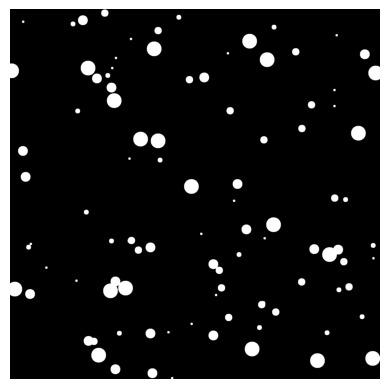
\includegraphics[width = 9.5cm, height = 9.5cm]{imagens_ft/granulometria.png}
	\caption{Exemplo de distribuição de objetos em uma imagem para aplicação de Granulometria.}
	\label{fig:granulometria}
\end{figure}

De acordo com \cite{r9}, uma boa Granulometria satisfaz os três itens abaixo. Seja $X$ uma imagem digital e $T^{(\lambda)}(X)$ a transformação que permite realizar uma Granulometria.

\begin{enumerate}
	\item a transformação morfológica deve ser anti--extensiva, ou seja, o conjunto transformado deve ser menor que o de origem. Matematicamente, 
	
	\begin{equation}
		\forall \lambda > 0, \; T^{(\lambda)}(X) \subset X \; \forall X.
	\end{equation}
	
	\item a transformação morfológica deve ser crescente. Matematicamente,
	
	\begin{equation}
		\forall \lambda > 0, \; Y \subset C \Rightarrow T^{(\lambda)}(X) \subset T^{(\lambda)}(Y) \; \forall X.
	\end{equation}
	
	\item consideramos a transformação de uma imagem $X$ a partir de duas transformações morfológica sucessiva de parâmetro respectivos $\lambda_1$ e $\lambda_2$. O resultado final deve ser idêntico qualquer que seja a sequência de transformações empregada. Além disso, o resultado deve ser idêntico ao obtido pela transformação de maior parâmetro $\lambda$:
	
	\begin{equation}
		\forall \lambda_1, \lambda_2 > 0, \; T^{(\lambda_1)}(T^{(\lambda_2)}(X)) = T^{(\lambda_2)}(T^{(\lambda_1)}(X)) = T^{sup(\lambda_1, \lambda_2)}(X) \; \forall X.
	\end{equation}
\end{enumerate}

Toda Granulometria pode ser representada: 

\begin{itemize}
	\item $\texttt{em números}$: consiste em numerar o conteúdo de cada peneiramento e representar o resultado em tamanho da peneira; 
	
	\item $\texttt{em medidas}$: consiste em uma tomada de peso do conteúdo de cada peneiramento. Essa massa é representada em função do tamanho de peneira.
\end{itemize}

Ambas as Granulometria podem ser representas graficamente. O eixo das abscissas representa os tamanho do Elemento Estruturante e no eixo das ordenadas fica o resultado obtido da Granulometria.

O processo de Granulometria é realizado utilizando as operações de Abertura, no entanto a Granulometria pode ser realizada com a operação de Fechamento a qual é chamada de Anti--Granulometria. 

A Granulometria por Abertura é implementada realizando sucessivas operações de Abertura com Elementos Estruturante de tamanhos gradualmente maiores. A diferença entre a imagem original e a imagem resultante da abertura é calculada, o tamanho do Elemento Estruturante é atualizado e o processo é repetido até que imagem $X_k$ seja igual $X_{k-1}$ ou até que o valor do crescimento do elemento estruturante seja atingido. Pode realizar qualquer tipo de Abertura Morfológica para implementar a Granulometria.

A Granulometria por Fechamento é implementada realizando sucessivas operações de Fechamento com Elementos Estruturante de tamanhos gradualmente maiores. A diferença entre o fechamento e a imagem original é calculada, o tamanho do Elemento Estruturante é atualizado e o processo é repetido até que imagem $X_k$ seja igual $X_{k-1}$ ou até que o valor do crescimento do elemento estruturante seja atingido. Pode utilizar qualquer tipo de Fechamento Morfológico para implementar a Granulometria.
